\documentclass[12pt,a4paper]{report}

% ---------- PACKAGES ----------
\usepackage[a4paper,margin=1in]{geometry}
\usepackage[utf8]{inputenc}
\usepackage[T1]{fontenc}
\usepackage{graphicx}
\graphicspath{{Pictures/}}
\usepackage{amsmath,amssymb}
\usepackage{booktabs}
\usepackage{longtable}
\usepackage{caption}
\usepackage{subcaption}
\usepackage{setspace}
\usepackage{fancyhdr}
\usepackage{xcolor}
\usepackage{listings}
\usepackage{titlesec}
\usepackage{enumitem}
\usepackage{tikz}
\usepackage[hidelinks]{hyperref}
\usepackage{float}                     % provides [H] = "put it HERE, no floating"
\usepackage[section]{placeins}         % \FloatBarrier + auto-barrier at every \section

% ---------- BIBLIOGRAPHY ----------
\renewcommand{\bibname}{References}

% ---------- TIKZ LIBRARIES ----------
\usetikzlibrary{arrows.meta, positioning, fit, backgrounds, shadows.blur, calc}

% ---------- CODE LISTING STYLE (single unified block) ----------
\lstset{
	basicstyle=\ttfamily\footnotesize,
	numbers=left,
	numberstyle=\tiny,
	breaklines=true,
	columns=fullflexible,
	frame=single,
	backgroundcolor=\color{gray!5},
	keywordstyle=\color{blue!70!black},
	commentstyle=\color{green!45!black},
	stringstyle=\color{red!60!black},
	showstringspaces=false,
	tabsize=2,
	language=Matlab
}

% ---------- PAGE STYLE ----------
\onehalfspacing
\pagestyle{fancy}
\fancyhf{}
\fancyhead[R]{\thepage}
\fancyhead[L]{Design, Analysis, and Modeling of a CNC Milling Spindle System}
\renewcommand{\headrulewidth}{0.4pt}

% ---------- TITLE ----------
\title{Design, Analysis, and Modeling of a CNC Milling Spindle System}
\author{}
\date{}

\begin{document}
	
	% =====================================================
	% TITLE PAGE
	% =====================================================
	\begin{titlepage}
		\centering
		
		{\large Addis Ababa Science and Technology University\par}
		{\large Department of Electromechanical Engineering\par}
		
		\vspace{0.8cm}
		
		
\includegraphics[width=3.5cm]{Pictures/AASTU_Logo_2b.jpg}
		
		\vspace{0.8cm}
		
		{\Large\bfseries Internship Project\par}
		
		\vspace{0.5cm}
		
		{\Large\bfseries
			Design, Analysis, and Modeling of a CNC Milling Spindle System
			\par}
		
		\vspace{1.5cm}
		
		{\large Submitted by:\par}
		\vspace{0.3cm}
		
		\begin{tabular}{rl}
			1. & Zahir Ahmed \quad ID: ETS1501/15 \\
			2. & Robera Kumsa \quad ID: ETS1162/15 \\
			3. & Samuel Tesfaye \quad ID: ETS1213/15 \\
			4. & Biniam Getahun \quad ID: ETS0350/14 \\
		\end{tabular}
		
		\vspace{1cm}
		
		{\large Submitted to:\par}
		Department of Electromechanical Engineering, AASTU\par
		
		\vspace{0.5cm}
		
		{\large Duration:\par}
		July to September 2026 G.C\par
		
		\vspace{0.5cm}
		
		{\large Organization:\par}
		Ethio-Engineering Group\par
		{\small Addis Ababa, Ethiopia\par}
		
		\vfill
		
		{\large September 15, 2026\par}
		
	\end{titlepage}
	
	% =====================================================
	% ABSTRACT
	% =====================================================
	\begin{abstract}
		This project presents the design, analysis, and modeling of a CNC milling spindle system as an integrated mechatronic system. The spindle is designed for high-speed operation with a maximum target speed of 5000 RPM, requiring consideration of mechanical strength, bearing support, motor selection, variable-speed operation, sensing, and control. The mechanical design includes the spindle shaft, bearing arrangement, housing, mounting components, and tool interface. Computer-aided design is used to develop the spindle assembly, while 
analytical hand calculations and a beam finite-element model are used to evaluate the structural performance of the spindle shaft, complemented by analytical checks of the housing and drawbar hardware.
		
		The electrical and power electronic aspects of the system are incorporated through the selection and modeling of a suitable AC spindle motor and variable frequency drive (VFD). The drive system is represented using an AC-DC-AC architecture consisting of a rectifier, DC link, and three-phase inverter, with pulse width modulation (PWM) used for motor control. A mathematical model of the motor-spindle system is developed based on the rotational dynamics of the system and is used to study the spindle response to speed commands and load disturbances. Closed-loop PID control is implemented using spindle speed feedback to regulate the operating speed.
		
		The automatic tool changer (ATC) and pneumatic drawbar are included as functional components of the overall spindle system. Their detailed mechanical and pneumatic analysis is outside the scope of the project; instead, they are incorporated into the supervisory control sequence. A programmable logic controller (PLC) is modeled as a supervisory layer responsible for sequencing and interlocking the spindle and tool-release operation. In particular, the PLC prevents tool release until the spindle has reached a safe standstill condition. Simulation results are used to evaluate the mechanical performance, motor-spindle dynamic response, PID speed regulation, and PLC-based supervisory interlocking. The project therefore integrates mechanical design, electrical drives, sensors, feedback control, and industrial automation into a unified CNC spindle mechatronic system.
		
		\vspace{0.5cm}
		\noindent\textbf{Keywords:} CNC Spindle, Automatic Tool Changer, Pneumatic Drawbar, Finite Element Analysis (FEA), Variable Frequency Drive (VFD), Pulse Width Modulation (PWM), Sinusoidal Pulse Width Modulation (SPWM), PID Control, PLC Interlocking, Mechatronics
	\end{abstract}
	
	% =====================================================
	% FRONT MATTER
	% =====================================================
	\tableofcontents
	\listoffigures
	\listoftables
	
	% =====================================================
	% CHAPTER 1: INTRODUCTION
	% =====================================================
	\chapter{Introduction}
	
	\section{Background of the Study}
	Computer numerical control (CNC) machine tools are widely used in modern manufacturing because they provide automated and precise control of machining operations. Among the major subsystems of a CNC milling machine, the spindle system is responsible for transmitting rotational power to the cutting tool and maintaining the required cutting speed during machining. The spindle therefore has a direct influence on machining performance, including cutting stability, dimensional accuracy, surface quality, and productivity.
	
	A CNC milling spindle is an electromechanical system in which mechanical, electrical, and control components operate together. Mechanically, the spindle consists of a rotating shaft supported by bearings and connected to a cutting tool. The shaft must withstand the combined effects of torque, bending loads, cutting forces, and rotational effects while maintaining sufficient stiffness and acceptable deformation. Machine-design principles for shafts, bearings, keys, power transmission components, and factors of safety are therefore essential to the spindle design \cite{ref1,ref2,ref3}.
	
	At high rotational speeds, however, static mechanical strength alone is not sufficient to characterize spindle performance. The dynamic behavior of the spindle-bearing system becomes increasingly important. Recent research has demonstrated that spindle speed, bearing stiffness, bearing clearance, imbalance, and other structural parameters can significantly affect spindle vibration and stability. Miao et al. developed a dynamic model of a CNC vertical milling-machine spindle system and showed that spindle speed and bearing parameters influence the vibration characteristics and stability of the system \cite{ref11}. Other studies have similarly investigated the natural frequencies, critical speeds, and imbalance response of high-speed spindle-bearing systems using finite element and dynamic modeling techniques \cite{ref12}.
	
	The spindle also requires a suitable electrical drive system to provide controlled rotational speed. An AC motor combined with a variable frequency drive can provide variable-speed operation by controlling the electrical frequency and voltage supplied to the motor. Electrical-machine theory provides the basis for understanding motor torque, speed, power, and operating characteristics, while power-electronic principles describe the conversion and control of electrical energy through rectifier, DC-link, and inverter stages \cite{ref4,ref5,ref6,ref7,ref8}. Recent work on CNC machining-center spindles has demonstrated the use of VFD-based induction-motor systems together with mathematical modeling and MATLAB/Simulink simulation for spindle speed regulation and load-response analysis \cite{ref13}.
	
	Speed regulation requires feedback and a control system capable of maintaining the desired spindle speed despite changes in operating conditions. A speed sensor such as a rotary encoder provides feedback of the actual spindle speed. The difference between the reference speed and measured speed is then processed by a PID controller to regulate the motor-drive command. Control-system theory provides the basis for analyzing the resulting closed-loop system in terms of stability, transient response, steady-state error, rise time, and settling time \cite{ref9}.
	
	In addition to continuous speed control, CNC equipment requires discrete supervisory functions to coordinate machine operations. Automatic tool changing is one such operation. The spindle must be brought to a suitable condition before the tool-release mechanism is activated. PLC-based control provides a practical method for implementing such sequencing and interlocking functions. Previous research has demonstrated the use of PLCs for CNC machine automation and tool-changing operations, including the coordination of machine inputs, outputs, and tool-change sequences \cite{ref14,ref15}.
	
	Therefore, the spindle considered in this project is treated as an integrated mechatronic system rather than as an isolated mechanical component. The mechanical structure, electrical drive, speed feedback, PID controller, and PLC supervisory logic are considered together. The design is based on a commercially available BT30 pneumatic tool-change spindle platform, which is modeled in CAD and analyzed across the mechanical, electrical, control, and automation domains. The primary design and analytical emphasis remains on the mechanical spindle, while the electrical, control, and automation subsystems are modeled at a level appropriate for demonstrating their interaction within the complete system.
	
	\section{Problem Statement}
	The spindle is one of the most important functional components of a CNC milling machine because it directly determines the rotational speed and power available to the cutting tool. Designing a spindle for high-speed operation requires more than selecting a rotating shaft. The shaft, bearings, housing, motor, drive system, sensors, and control system must operate together while maintaining acceptable mechanical and dynamic performance.
	
	A mechanically adequate spindle may still experience poor performance if its motor-drive system cannot provide the required speed or if the control system cannot maintain the desired speed under changing cutting loads. Similarly, a speed controller alone cannot guarantee safe tool-changing operation. A tool-release command issued while the spindle is still rotating can result in an unsafe operating condition. Consequently, continuous speed regulation and discrete machine sequencing must be considered as separate but coordinated control functions.
	
	Previous research has addressed different aspects of CNC spindle systems, including spindle-bearing dynamics, finite element modeling, motor-drive control, and PLC-based automation. For example, dynamic spindle studies have investigated the influence of bearing characteristics and spindle speed on vibration behavior \cite{ref11}, while VFD-based spindle research has demonstrated mathematical and MATLAB/Simulink models for speed control of AC motor-driven CNC spindles \cite{ref13}. PLC-based research has also demonstrated the use of programmable controllers for CNC automation and tool-change operations \cite{ref14,ref15}. These functions are, however, frequently treated in isolation from one another.
	
	The problem addressed in this project is therefore the design and system-level modeling of a CNC milling spindle that combines the mechanical spindle structure with an electrical drive, speed feedback, PID control, and PLC-based supervisory interlocking. The project demonstrates how these subsystems operate together within a single, coherent mechatronic system.
	
	\section{Objectives}
	\subsection{General Objective}
	To design, analyze, and model a CNC milling spindle system as an integrated mechatronic system incorporating mechanical design, electrical drive modeling, PID speed control, sensing, and PLC-based supervisory interlocking.
	
	\subsection{Specific Objectives}
	The specific objectives of the project are to:
	\begin{enumerate}[label=\arabic*.]
		\item Design the main mechanical components of a CNC milling spindle capable of operating at a target maximum speed of 5000 RPM.
		\item Determine the required spindle torque, power, shaft dimensions, and bearing loads based on the specified operating and cutting conditions.
		\item Develop a three-dimensional CAD model and assembly of the spindle system using SolidWorks.
		\item Analyze the mechanical behavior of the spindle components using analytical calculations and finite element analysis.
		\item Evaluate spindle stress, deformation, and factor of safety under the specified loading conditions.
		\item Select and model a suitable AC spindle motor and variable frequency drive for the required operating speed.
		\item Develop a mathematical model representing the rotational dynamics of the motor-spindle system.
		\item Develop a representation of the power-electronic drive, including the rectifier, DC link, inverter, and PWM-based switching.
		\item Develop a closed-loop PID speed-control system using spindle speed feedback.
		\item Evaluate the dynamic response of the spindle under speed commands and load disturbances.
		\item Develop a PLC-based supervisory sequence for spindle stopping and tool-release operation.
		\item Implement an interlocking condition that prevents pneumatic drawbar activation until the spindle reaches the required safe-speed condition ($\leq 5$~RPM).
		\item Compare the simulated spindle/tool-release behavior with and without PLC supervisory interlocking.
		\item Demonstrate the integration of mechanical, electrical, sensing, control, and automation subsystems within the CNC spindle system.
	\end{enumerate}
	
	\section{Scope and Limitation}
	The project covers the design, analysis, and system-level modeling of a CNC milling spindle intended for operation up to 5000 RPM. The mechanical scope includes the spindle shaft, bearing arrangement, housing and mounting components, tool interface, and the other major structural components required for the spindle assembly. CAD modeling is performed using SolidWorks, while analytical calculations and FEA are used to evaluate the mechanical performance of the design.
	
	The electrical scope covers the selection and functional modeling of an AC motor and variable frequency drive. The drive is represented at the system level using the conventional rectifier, DC-link, and inverter structure. PWM, particularly sinusoidal PWM, is the modulation method used by the inverter to control the motor supply. The project does not include detailed semiconductor-device design, thermal analysis of IGBTs, detailed electromagnetic design of the motor, or physical construction of a VFD.
	
	The control scope includes mathematical modeling of the motor-spindle dynamics and closed-loop PID speed control. A speed-feedback sensor provides the measured spindle speed to the controller. The performance of the controller is evaluated using simulated speed commands and load disturbances.
	
	The automatic tool changer and pneumatic drawbar are treated as functional components of the overall CNC spindle system. They are not subjected to detailed mechanical, pneumatic, fluid-dynamic, or manufacturing analysis. Instead, the pneumatic drawbar is represented as a simplified actuator in the supervisory-control model, and its operation is coordinated by the PLC according to the spindle operating state.
	
	The PLC component of the project is modeled at the supervisory level. The PLC is responsible for sequencing and interlocking operations, while the PID controller provides continuous spindle-speed regulation. The PLC handles discrete logic for operations such as spindle stopping, safe-speed verification, and tool-release permission. The project does not involve the construction of a complete industrial PLC control panel or physical implementation of the automatic tool changer.
	
	\section{Methodology Overview}
	The methodology begins with the identification of the main operating requirements of the CNC milling spindle, including the target rotational speed, mechanical loading conditions, required torque, and power requirements. These requirements establish the initial dimensions and configuration of the spindle system.
	
	The mechanical design is developed through analytical calculations based on established machine-design and mechanics principles. Shaft loading is evaluated under bending and torsional conditions, while bearing loads and other relevant mechanical requirements are determined from the specified operating conditions. The resulting geometry is developed as a three-dimensional CAD assembly in SolidWorks.
	
	Finite element analysis is subsequently performed on the critical mechanical components. The FEA model evaluates stress and deformation under the defined loading conditions. The analytical and numerical results are compared to confirm that the design satisfies the required structural conditions.
	
	The electrical subsystem is developed by selecting a spindle motor and representing its connection to a variable frequency drive. The drive is modeled using a functional AC-DC-AC architecture consisting of a rectifier, DC link, and inverter. PWM represents the generation of controlled switching signals for motor operation. The electrical and mechanical subsystems are combined to form a mathematical model of the motor-spindle system.
	
	A closed-loop speed controller is developed using PID control. The reference spindle speed is compared with the measured speed, and the resulting error is processed by the controller to generate the motor-drive command. The model is simulated to evaluate speed tracking, transient response, steady-state error, and response to changes in load torque.
	
	Finally, a supervisory PLC model is developed to coordinate the spindle and tool-release sequence. When a tool-release request is received, the PLC first commands the spindle to stop and verifies that the spindle has reached the defined safe-speed condition. Only after this condition is satisfied is the pneumatic drawbar permitted to activate. The resulting behavior is compared with a system without PLC interlocking to demonstrate the effect of supervisory control on safe tool-release operation.
	
	The overall methodology can therefore be represented as:
	
	\begin{figure}[htbp]
		\centering
		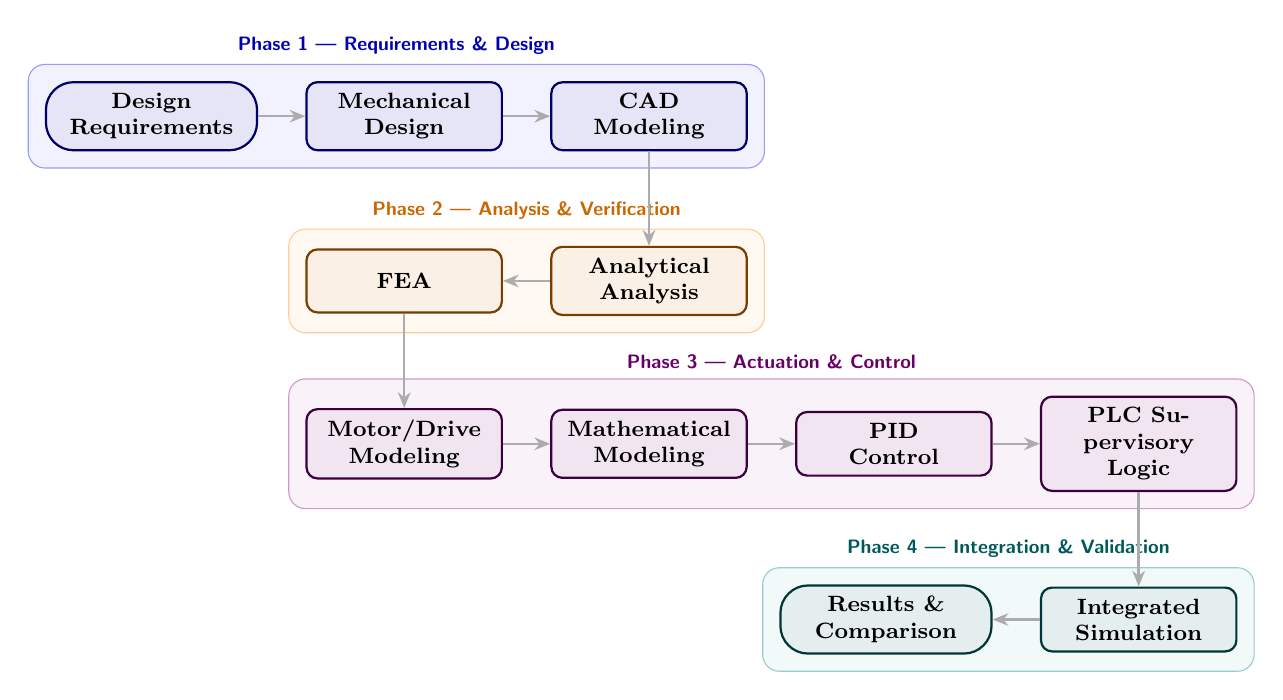
\begin{tikzpicture}[
			node distance=6mm and 6mm,
			every node/.style={font=\footnotesize\sffamily},
			step/.style={
				rectangle, rounded corners=4pt,
				draw=#1!60!black, fill=#1!10,
				line width=0.8pt, inner sep=4pt,
				minimum height=8mm, text width=22mm,
				align=center, font=\footnotesize\bfseries
			},
			terminal/.style={
				step=#1, rounded corners=10pt, text width=24mm
			},
			arrow/.style={
				-{Stealth[length=2mm,width=1.6mm]},
				line width=0.9pt, draw=gray!65
			},
			phaselabel/.style={
				font=\scriptsize\bfseries\sffamily, text=#1
			}
			]
			
			% Row 1
			\node[terminal=blue!70!black] (dr)  {Design\\Requirements};
			\node[step=blue!70!black, right=of dr] (md) {Mechanical\\Design};
			\node[step=blue!70!black, right=of md] (cad){CAD\\Modeling};
			
			% Row 2
			\node[step=orange!80!black, below=12mm of cad] (aa) {Analytical\\Analysis};
			\node[step=orange!80!black, left=of aa]          (fea){FEA};
			
			% Row 3
			\node[step=violet!80!black, below=12mm of fea] (mdm){Motor/Drive\\Modeling};
			\node[step=violet!80!black, right=of mdm]      (mm) {Mathematical\\Modeling};
			\node[step=violet!80!black, right=of mm]       (pid){PID\\Control};
			\node[step=violet!80!black, right=of pid]      (plc){PLC Supervisory\\Logic};
			
			% Row 4
			\node[step=teal!70!black, below=12mm of plc] (is){Integrated\\Simulation};
			\node[terminal=teal!70!black, left=of is]    (rc){Results \&\\Comparison};
			
			% Arrows
			\draw[arrow] (dr)  -- (md);
			\draw[arrow] (md)  -- (cad);
			\draw[arrow] (cad) -- (aa);
			\draw[arrow] (aa)  -- (fea);
			\draw[arrow] (fea) -- (mdm);
			\draw[arrow] (mdm) -- (mm);
			\draw[arrow] (mm)  -- (pid);
			\draw[arrow] (pid) -- (plc);
			\draw[arrow] (plc) -- (is);
			\draw[arrow] (is)  -- (rc);
			
			% Phase backgrounds
			\begin{scope}[on background layer]
				\node[fit=(dr)(md)(cad), fill=blue!5, draw=blue!40,
				rounded corners=6pt, inner sep=6pt,
				label={[phaselabel=blue!70!black]above:Phase 1 --- Requirements \& Design}] {};
				\node[fit=(aa)(fea), fill=orange!5, draw=orange!40,
				rounded corners=6pt, inner sep=6pt,
				label={[phaselabel=orange!80!black]above:Phase 2 --- Analysis \& Verification}] {};
				\node[fit=(mdm)(mm)(pid)(plc), fill=violet!5, draw=violet!40,
				rounded corners=6pt, inner sep=6pt,
				label={[phaselabel=violet!80!black]above:Phase 3 --- Actuation \& Control}] {};
				\node[fit=(is)(rc), fill=teal!5, draw=teal!40,
				rounded corners=6pt, inner sep=6pt,
				label={[phaselabel=teal!70!black]above:Phase 4 --- Integration \& Validation}] {};
			\end{scope}
			
		\end{tikzpicture}
		\caption{Overall methodology: from design requirements to validated results.}
		\label{fig:methodology}
	\end{figure}
	
	% =====================================================
	% CHAPTER 2: LITERATURE REVIEW
	% =====================================================
	\chapter{Literature Review}
	
	\section{Spindle Mechanics and Bearing Dynamics}
	The spindle is a critical rotating subsystem of a CNC milling machine because it transmits mechanical power from the drive system to the cutting tool while maintaining the required rotational speed and positional stability. Its mechanical design must provide adequate strength and stiffness while limiting deformation and vibration during operation. The design of shafts, bearings, keys, power-transmission components, and supporting structures is established using standard machine-design and mechanics principles \cite{ref1,ref2,ref3}.
	
	For a spindle shaft, the applied loading is a combination of torsional and bending loading. The transmitted motor torque produces torsional stress, while cutting forces acting at the tool produce bending moments. The combined loading is considered when determining the shaft dimensions and evaluating the resulting factor of safety. The shaft must also maintain sufficient stiffness so that excessive deflection does not affect the position of the cutting tool.
	
	Bearing selection is equally important because the bearings support the rotating spindle while transmitting radial and axial loads to the housing. At high rotational speeds, bearing stiffness, preload, clearance, and dynamic behavior influence the overall response of the spindle. Consequently, bearing selection is considered together with spindle geometry and operating speed.
	
	Recent research has demonstrated the importance of considering spindle and bearing dynamics together. Miao et al. developed a dynamic model of a CNC vertical milling-machine spindle system incorporating nonlinear bearing restoring forces, radial clearance, and time-varying bearing stiffness \cite{ref11}. Their results showed that spindle speed and bearing parameters influence the vibration characteristics and stability of the spindle system. The study also considered factors such as pulley eccentricity, tool overhang, and bearing arrangement, demonstrating the interaction between spindle configuration and dynamic behavior.
	
	Other research has used finite element models to investigate the vibration characteristics of high-speed spindle-bearing systems. Such studies have examined natural frequencies, mode shapes, critical speeds, and unbalanced response, with bearing stiffness identified as an important factor in the dynamic characteristics of the spindle \cite{ref12}. These findings indicate that the spindle is evaluated not only according to static strength requirements but also according to its dynamic operating characteristics.
	
	A dynamic model of a spindle-bearing system has also been developed using finite element representation of the spindle shaft and tool-holder assembly. The model considered the interaction between the spindle shaft, bearings, housing, and cutting forces and was used to investigate frequency-response and time-domain behavior under different spindle speeds and cutting conditions \cite{ref16}. The agreement between simulated and experimental responses demonstrated the usefulness of dynamic spindle models for evaluating machine-tool performance.
	
	For the present project, these studies establish the importance of integrating shaft design, bearing support, loading, and dynamic behavior into a single design process, which is the approach adopted in Chapter 3.
	
	\section{Electrical Drives in Machining}
	The spindle motor and its associated drive form the electrical portion of the spindle system. Unlike a conventional fixed-speed motor application, a CNC spindle requires controlled variation of rotational speed according to the machining operation. Electrical-machine theory provides the basis for selecting an appropriate motor, while power-electronic drives provide the means of controlling the voltage and frequency supplied to the motor \cite{ref4,ref5,ref6,ref7,ref8}.
	
	AC motors are widely applicable to industrial variable-speed drive systems because of their robustness and compatibility with electronic power conversion. For an induction motor, the synchronous speed is related to the electrical supply frequency and the number of motor poles by
	\begin{equation}
		N_s=\frac{120f}{P}
	\end{equation}
	where $N_s$ is the synchronous speed in revolutions per minute, $f$ is the electrical supply frequency, and $P$ is the number of poles. The actual rotor speed differs from synchronous speed because of slip \cite{ref4,ref5,ref6}. This relationship makes frequency control the primary method for variable-speed operation of induction-motor-driven systems. The present project uses a permanent-magnet synchronous (PMSM/BLDC-family) AC servo motor instead, discussed in Section~\ref{sec:machine_selection}; the synchronous-speed relationship above still governs the inverter's output-frequency requirement.
	
	A variable frequency drive provides the required electrical conversion and control. A conventional AC drive is represented by an AC-DC-AC structure consisting of a rectifier, DC link, and inverter. The rectifier converts the input AC supply into DC, the DC link smooths and stores electrical energy, and the inverter generates a controlled output for the motor. Power-electronic switching devices such as IGBTs are controlled using PWM techniques to synthesize the required output voltage waveform \cite{ref7,ref8}.
	
	PWM provides a practical method of controlling the inverter output by rapidly switching the power devices. In sinusoidal PWM, a sinusoidal reference waveform is compared with a high-frequency carrier signal to generate the switching pulses. The frequency of the reference signal is associated with the desired motor electrical frequency, while the modulation index influences the output voltage magnitude. More advanced approaches, including space-vector PWM and vector control, have also been extensively investigated for AC motor drives.
	
	Recent research has directly applied VFD-based control to CNC machining-center spindles. A recent study developed a rotational model of a CNC spindle incorporating an AC motor, transmission system, and rotating spindle, and developed an induction-motor model in the $d$-$q$ reference frame. The resulting VFD-based system was implemented and evaluated using MATLAB/Simulink under speed commands and torque-load disturbances \cite{ref13}. The study demonstrates the suitability of mathematical and simulation-based approaches for analyzing variable-speed CNC spindle drives.
	
	PLC-based spindle drive systems have also been investigated in high-speed machine applications. Yin et al. developed a high-speed spindle drive-control system using a PLC, frequency converter, speed feedback sensor, and PID closed-loop control. The system used spindle-speed feedback to regulate the motor speed and employed the PLC for real-time signal acquisition and system control \cite{ref17}.
	
	These studies support the use of an AC motor, VFD, speed sensor, and closed-loop controller in the present project, and the system described in Chapter 3 follows this architecture.
	
	\section{Machining Dynamics and Control}
	The spindle operates under continuously changing mechanical conditions during machining. Changes in cutting conditions modify the torque required from the motor, causing variations in spindle speed if the drive system is unable to compensate for the disturbance. For this reason, mathematical modeling and closed-loop speed control are essential parts of an integrated spindle system.
	
	The mechanical behavior of the spindle is represented by a rotational dynamic equation:
	\begin{equation}
		J\frac{d\omega}{dt}=T_m-T_L-B\omega
	\end{equation}
	where $J$ represents the equivalent rotational inertia of the motor-spindle system, $\omega$ represents angular velocity, $T_m$ is the motor torque, $T_L$ is the external load torque, and $B$ represents the equivalent viscous damping coefficient. This model provides a representation of the relationship between motor torque, mechanical loading, and spindle speed.
	
	The mathematical model is incorporated into a feedback-control system. In closed-loop speed control, the desired spindle speed is compared with the measured spindle speed. The difference between these values forms the control error. A PID controller processes this error and produces a control command for the motor-drive system \cite{ref9}.
	
	The PID controller is represented by
	\begin{equation}
		u(t)=K_pe(t)+K_i\int e(t)\,dt+K_d\frac{de(t)}{dt}
	\end{equation}
	where $e(t)$ is the speed error, $K_p$ is the proportional gain, $K_i$ is the integral gain, and $K_d$ is the derivative gain. The proportional term responds to the magnitude of the current error, the integral term eliminates persistent steady-state error, and the derivative term responds to changes in the error.
	
	Recent research has emphasized the importance of dynamic modeling in CNC spindle systems. Miao et al. developed a detailed spindle dynamic model and examined its behavior under different spindle speeds, bearing parameters, imbalance conditions, and tool configurations \cite{ref11}. Their work demonstrates that spindle dynamics significantly affect machining stability and accuracy. Another recent spindle-modeling study used a system-level modeling approach to investigate spindle dynamics and energy behavior, demonstrating the usefulness of simulation models for studying the response of spindle systems under different operating conditions.
	
	Speed-control research has also demonstrated the use of feedback controllers with spindle drive systems. In the VFD-based CNC spindle study discussed above, a closed-loop controller was used to regulate spindle speed and evaluate the dynamic response of the spindle under torque disturbances \cite{ref13}. Experimental work on high-speed spindle drive systems has similarly combined frequency converters, speed feedback, PLC control, and PID-based closed-loop regulation to maintain the required spindle speed \cite{ref17}.
	
	In the present project, PID control is therefore used as the \textbf{continuous control layer} responsible for maintaining the desired spindle speed. The PLC does not replace this controller. Instead, it provides a separate \textbf{supervisory control layer} for discrete operations and safety interlocking. This distinction is important because speed regulation and tool-change sequencing represent different types of control problems.
	
	During tool release, for example, the PID controller regulates the spindle at its commanded speed while having no knowledge of whether a tool-release operation is safe. A PLC supervisory controller monitors the tool-release request and spindle-speed feedback, commands the spindle to stop, verifies the spindle speed is below the 5~RPM safety threshold, and only then permits the pneumatic drawbar to activate. Research on CNC tool-changing has demonstrated the use of PLC programming to coordinate automated tool-change operations in CNC machine systems \cite{ref14}, while other CNC automation research has demonstrated PLC-based coordination of machine inputs, outputs, motor control, and automatic loading and unloading \cite{ref15}.
	
	The proposed control architecture therefore combines continuous PID speed regulation with discrete PLC supervisory logic. This provides a complete representation of the CNC spindle as a mechatronic system rather than treating the mechanical spindle, motor drive, and automation functions as independent systems.
	
	% =====================================================
	% CHAPTER 3: SYSTEM DESIGN
	% =====================================================
	\chapter{System Design}
	
	\section{Mechanical Design}\label{sec:mech_design}
	This section follows the standard machine-design sequence: establish the design loads
	(Section~\ref{sec:load_analysis}), select and size each machine element against those loads
	(Sections~\ref{sec:machine_elements}--\ref{sec:shaft_design}), and describe how the assembly is realized
	(Section~\ref{sec:fab_assembly}). The design is based on a commercially available BT30
	pneumatic tool-change spindle platform, modeled in SolidWorks and analyzed below.
	
	\subsection{Load Analysis}\label{sec:load_analysis}
	
	\subsubsection{Design Cutting Scenario}\label{sec:baseline_cutting}
	The design loads for the shaft, bearings, and drive motor are established from a roughing
	scenario using Aluminum 6061-T6 as the workpiece material and a 10~mm diameter, 3-flute
	solid carbide end mill. Aluminum represents a realistic roughing condition for a
	light-industrial BT30 spindle and remains within the load capacity of the deep-groove
	bearings and the 5M timing belt drive. The design parameters are:
	
	\begin{itemize}
		\item Workpiece material: Aluminum 6061-T6
		\item Tool: $\varnothing 10$~mm solid carbide end mill, $z = 3$ flutes
		\item Spindle speed: $N = 5000$~RPM (rated maximum)
		\item Feed per tooth: $f_z = 0.05$~mm/tooth
		\item Axial depth of cut: $a_p = 3.0$~mm
		\item Radial depth of cut: $a_e = 5.0$~mm (50\% radial engagement)
	\end{itemize}
	
	The specific cutting force is taken as $k_c = 900$~N/mm$^2$, at the upper end of the
	range reported for 6061-T6 in machining handbooks (typically 600--800~N/mm$^2$). Using
	the conservative figure biases every downstream force, stress, bearing life, and shaft
	dimension on the safe side.
	
	Cutting speed and feed rate follow directly:
	\begin{align}
		V_c &= \frac{\pi D N}{1000} = \frac{\pi (10)(5000)}{1000} \approx 157.1~\text{m/min} \\
		v_f &= f_z \, z \, N = (0.05)(3)(5000) = 750~\text{mm/min}
	\end{align}
	
	\subsubsection{Material Removal Rate and Average Cutting Power}\label{sec:mrr_power}
	The material removal rate is:
	\begin{equation}
		\text{MRR} = a_p \, a_e \, v_f = (3)(5)(750) = 11{,}250~\text{mm}^3\text{/min} = 187.5~\text{mm}^3\text{/s}
	\end{equation}
	Taking $k_c = 900$~N/mm$^2$ and converting to specific cutting energy
	$u = k_c / 1000 = 0.9$~J/mm$^3$, the average cutting power at the spindle is:
	\begin{equation}
		P_{c,avg} = u \cdot \text{MRR} = (0.9)(187.5) \approx 169~\text{W}
	\end{equation}
	This average power figure is the basis for continuous motor power sizing (Section~\ref{sec:motor_sizing}).
	
	\subsubsection{Peak Cutting Force and Spindle Torque (Torsion)}\label{sec:peak_force_torque}
	Average power alone understates the instantaneous structural load, since milling is an
	intermittent process. Using a simplified Kienzle-type model with $h \approx f_z$, the peak
	tangential force on a single engaged tooth is:
	\begin{equation}
		F_{c,peak} = k_c \, a_p \, f_z = (900)(3)(0.05) = 135~\text{N}
	\end{equation}
	The tooth engagement angle for $a_e/D = 50\%$ is $\phi_{a_e} = \arccos(1 - 2a_e/D) = 90^\circ$,
	compared to a tooth pitch angle of $360^\circ/z = 120^\circ$. Since $\phi_{a_e} < 360^\circ/z$,
	only one tooth is engaged at any instant, confirming an intermittent, single-tooth worst-case
	loading condition. The corresponding peak spindle torque (the shaft's \emph{torsional} load)
	is:
	\begin{equation}
		T_{peak} = F_{c,peak} \cdot \frac{D}{2} = (135)(0.005) = 0.675~\text{N}\cdot\text{m}
	\end{equation}
	
	\subsubsection{Overhung Load, Bending, and Bearing Reactions}\label{sec:overhung_bending}
	The end mill acts at the end of a cantilevered overhang beyond the front (nose) bearing, so
	$F_{c,peak}$ also produces a \emph{bending} load on the shaft, and amplifies the radial load
	seen by each bearing beyond the applied cutting force itself -- this is the standard
	overhung-load model used in bearing catalogs \cite{ref1}. Modeling the shaft as simply
	supported between the front and rear bearings (span $L_1$) with the tool tip overhanging the
	front bearing by $L_2$: $L_1 = 49.7$~mm is the point-to-point distance between the front and
	rear bearing-seat shoulder centers, measured directly from the CAD geometry and verified
	against an independent axis-to-axis cross-check. The overhang $L_2 = 123.85$~mm combines a
	38.85~mm nose-to-front-bearing distance with the tool holder's own projection. The tool
	holder is a \textbf{BT30-ER20-70} with a 70~mm gauge-length projection, plus an additional
	15~mm allowance for the 10~mm end mill's stick-out beyond the collet face. Since the
	tool holder is a physically separate component whose body sits almost entirely outside the
	housing (protruding from the spindle nose), its full projection is additive to the
	housing-side measurement:
	$L_2 = 38.85 + 70 + 15 = 123.85$~mm. The bearing reactions and peak bending moment are:
	\begin{align}
		R_{front} &= F_{c,peak}\cdot\frac{L_1+L_2}{L_1} = 135 \times \frac{173.55}{49.7} \approx 471.4~\text{N} \\
		R_{rear} &= F_{c,peak}\cdot\frac{L_2}{L_1} = 135 \times \frac{123.85}{49.7} \approx 336.4~\text{N} \quad (\text{reversed direction}) \\
		M_{max} &= F_{c,peak}\cdot L_2 = 135 \times 123.85 \approx 16{,}720~\text{N}\cdot\text{mm} = 16.72~\text{N}\cdot\text{m} \quad (\text{at the front bearing})
	\end{align}
	Two points follow directly: (i) the front bearing radial load is more than triple the applied
	cutting force purely due to the overhang geometry, and (ii) the rear bearing reaction
	\emph{reverses direction} relative to the applied load -- deep-groove ball bearings tolerate
	this radial reversal without issue. These values feed directly into the bearing
	life check (Section~\ref{sec:bearing_design}) and the shaft diameter calculation (Section~\ref{sec:shaft_design}).
	
	\begin{figure}[H]
		\centering
		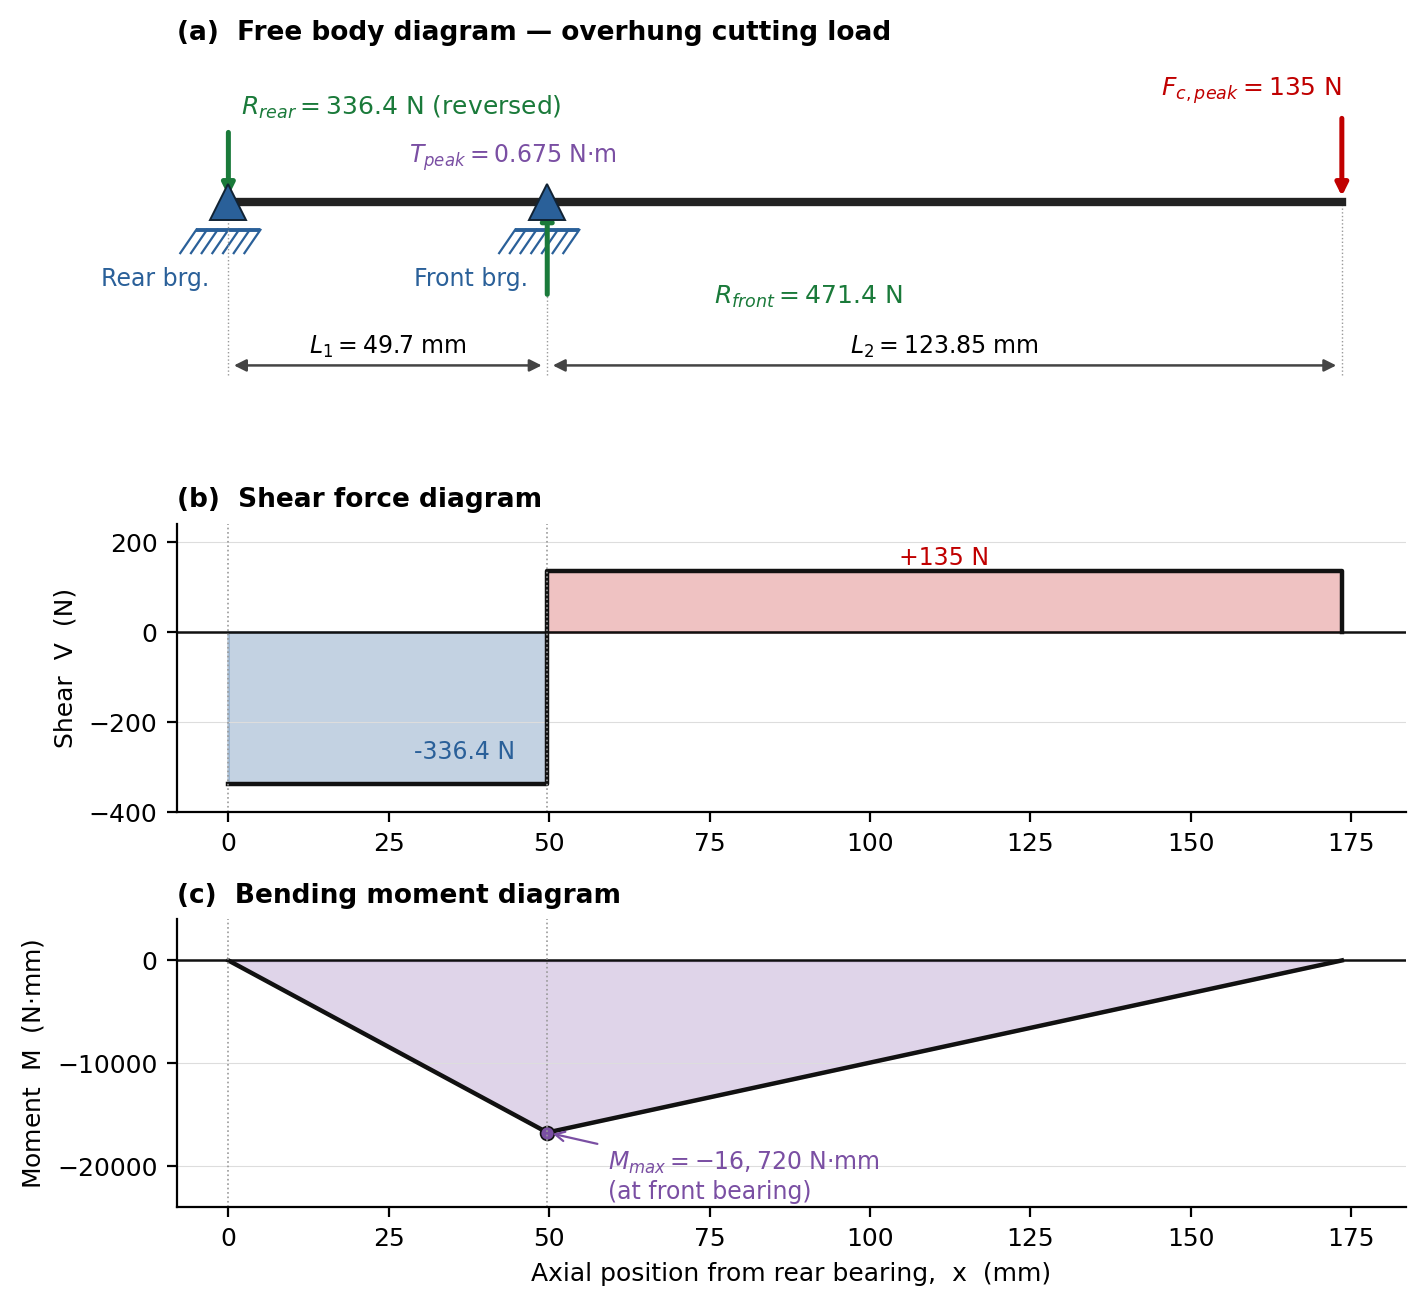
\includegraphics[width=0.85\textwidth]{Pictures/fig_3_1_shaft_fbd.png}
		\caption{Overhung-load free body diagram and shear/bending-moment diagram for the spindle shaft.}
		\label{fig:shaft_fbd}
	\end{figure}
	
	\subsubsection{Pneumatic Drawbar Axial Load}\label{sec:drawbar_load}
	The tool-change (drawbar release) event applies a separate, large axial load through the
	spindle centerline, unrelated to the cutting load above. The actuator is a pneumatic
	cylinder rated to deliver $F_{cyl} = 2940$~N (300~kgf) at a supply pressure of
	$0.8$~MPa \cite{ref1}. The theoretical force from the bore area alone
	($A = \pi D_{bore}^2/4 = \pi(80)^2/4 = 5026.5$~mm$^2$) is:
	\begin{equation}
		F_{cyl,max} = P \cdot A = (0.8)(5026.5) \approx 4021~\text{N}
	\end{equation}
	The ratio $F_{cyl}/F_{cyl,max} = 2940/4021 \approx 0.731$ is consistent with typical
	pneumatic-cylinder mechanical efficiency of 70--75\% once seal friction and internal flow
	losses are accounted for; the manufacturer's rated force is the \emph{net} output after
	those losses, while the bore-area calculation gives the theoretical maximum. The design
	drawbar load case used in Sections~\ref{sec:machine_elements} and \ref{sec:bearing_design} is
	therefore bracketed between $2940$~N (rated, realistic) and $4021$~N (theoretical maximum,
	worst case).
	
	\subsubsection{Motor Power and Torque Requirement}\label{sec:motor_sizing}
	Sizing the drive motor requires converting spindle-side average power/torque to the motor
	side across the 5M timing belt (sized in Section~\ref{sec:belt_pulley}). The manufacturer's
	product specification for the pulley pair gives a motor pulley of 50 teeth and a spindle
	pulley of 30 teeth -- the \emph{motor} pulley is larger, so the motor runs \emph{slower}
	than the spindle, a step-up ratio of $50/30 = 5/3 \approx 1.667\!:\!1$ (spindle:motor).
	The direction of the ratio is confirmed by the motor's rated speed: a 1~kW-class AC servo
	is near-universally rated at $\sim$3000~RPM, and $5000 \times 30/50 = 3000$~RPM matches
	that exactly. The reverse direction (30~T motor, 50~T spindle) would require the motor to
	run at 8333~RPM to reach the spindle's rated 5000~RPM, which no motor in this class can
	do -- so the 50:30 configuration is the only one physically consistent with the specified
	hardware.
	
	With a belt efficiency of $\eta = 0.90$ and a service factor of $SF = 1.5$ (tool wear,
	chip evacuation, roughing dynamics):
	\begin{equation}
		P_{motor} \geq \frac{P_{c,avg}}{\eta}\times SF = \frac{169}{0.90}\times 1.5 \approx 281~\text{W}
	\end{equation}
	A motor rated at 300--400~W (continuous) is therefore sufficient for the aluminum-roughing
	scenario alone. The spindle kit is equipped with a \textbf{1000~W AC servo motor with
		brake}, providing a substantial margin that covers steel and heavier cuts beyond the
	aluminum baseline analyzed here. The motor is specified in its \textbf{220~V} input-rated
	variant, matching Ethiopia's 230~V/50~Hz single-phase mains standard directly with no
	step-down transformer required (Section~\ref{sec:machine_selection} discusses this further). At 1000~W the motor
	is sized at $3.5\times$ the calculated minimum, and its rated 3000~RPM speed coincides
	precisely with the spindle's top operating speed through the 5:3 belt ratio.
	
	\subsection{Design of Machine Elements}\label{sec:machine_elements}
	This section covers the principal load-carrying and functional elements of the spindle: the
	housing and tool interface, the Belleville washer stack, the drawbar and pull stud, the
	retention hardware, the spindle key, and the floating puller assembly. Standard fasteners
	that are selected by standard practice are not individually calculated here; the elements
	below are the ones that govern performance, safety, or accuracy.
	
	\paragraph{Spindle housing and tool interface.} The housing is 7075-T6 aluminum,
	selected for its high strength-to-weight ratio relative to 6061, which reduces
	rotating/reciprocating mass without a proportional cost increase for a low-volume build.
	The BT30 taper with ER20 collet is a fixed interface dictated by the spindle platform.
	ER20 covers a 1--13~mm clamping range, which accommodates the 10~mm end mill used in the
	design scenario (Section~\ref{sec:load_analysis}).
	
	\paragraph{Belleville washer stack.} Disc (Belleville) springs are used in place of a
	conventional coil spring because the drawbar must generate a large clamping force over a
	very short axial travel (a few millimeters) within the tight radial envelope of the spindle
	bore -- Belleville washers have the highest force-per-unit-volume of the common spring types
	and are the standard solution for this application \cite{ref1}. Stacking washers
	\emph{in parallel} (same orientation) increases the delivered force for a given deflection;
	stacking \emph{in series} (alternating orientation) increases deflection at a given force.
	The stack is configured to deliver the clamping force required to resist tool pull-out under
	the peak cutting force computed in Section~\ref{sec:peak_force_torque}.
	
	\paragraph{Drawbar and pull stud.} The pull stud threads into the tool holder's retention
	knob per the BT30 standard and is pulled rearward by the Belleville stack to seat the taper.
	The M12 pull stud is the standard size for this tooling class.
	
	\paragraph{Retention hardware.} The drawbar is retained by an M8 lock screw and locknut,
	reacting a shear load equal to the drawbar force via $\tau = F/A_{shear}$ with
	$A_{shear} = \pi d_{minor}^2/4$ \cite{ref1}. For M8 ($d_{minor} = 6.647$~mm,
	$A_{shear} = 34.71$~mm$^2$):
	
	\begin{table}[htbp]
		\centering
		\caption{Shear stress and factor of safety in the M8 drawbar retention hardware.}
		\label{tab:retention_hardware}
		\begin{tabular}{lccc}
			\toprule
			Condition & Axial Force (N) & Shear Stress $\tau$ (MPa) & Factor of Safety \\
			\midrule
			Rated ($F_{cyl}$) & 2940 & 84.7 & 2.18 \\
			Theoretical maximum ($F_{cyl,max}$) & 4021 & 115.9 & 1.60 \\
			\bottomrule
		\end{tabular}
	\end{table}
	
	\noindent Against a typical allowable shear stress of
	$\tau_{allow} \approx 0.577\,S_y \approx 185$~MPa for a common-grade fastener \cite{ref1},
	the M8 retention hardware clears both load cases with margin.
	
	\paragraph{Spindle key.} A 5~mm $\times$ 30~mm parallel key is used on the shaft, sized per
	standard key tables for a $\sim$20~mm shaft (Section~\ref{sec:shaft_design}). Checking it
	against the peak torque from Section~\ref{sec:peak_force_torque} ($T_{peak} = 675$~N$\cdot$mm)
	with key width $b=5$~mm, height $h=5$~mm, length $L=30$~mm, and shaft radius $r=10$~mm \cite{ref1}:
	\begin{align}
		\tau_{key} &= \frac{T_{peak}}{b\,L\,r} = \frac{675}{(5)(30)(10)} = 0.45~\text{MPa} \\
		\sigma_{bearing} &= \frac{2\,T_{peak}}{h\,L\,r} = \frac{2(675)}{(5)(30)(10)} = 0.9~\text{MPa}
	\end{align}
	Both are trivial compared to a typical key-stock allowable ($\tau_{allow} \sim 100$~MPa).
	The key's function is therefore \emph{not} torque capacity -- it is
	\textbf{eliminating slip} so that the encoder's measured position tracks the true spindle
	position, which is a requirement for the closed-loop control in Section~\ref{sec:controller_design}.
	
	\paragraph{Floating puller assembly.} The pneumatic cylinder drives a puller plate along two
	guide rods, compressing the return springs. The load is transferred through the puller rod
	into a bearing tube that houses a bearing, allowing the non-rotating puller rod to press
	axially on the rotating drawbar and pull disc without transmitting rotation into the
	stationary actuation hardware. A lower plate is the fixed reaction structure: it carries the
	axial release force directly into the housing, isolating the spindle bearings from the
	drawbar release load. A flanged bolt and lower stop set the stroke and prevent
	over-extension of the mechanism, and a load-spreading washer distributes the cylinder
	mounting load.
	

	
	\subsection{Belt and Pulley Design}\label{sec:belt_pulley}
	The 5M (5~mm pitch) HTD timing belt drive uses 50 teeth on the (slower) motor pulley and
	30 teeth on the (faster) spindle pulley, per the manufacturer's product specification. The
	pitch diameters are:
	\begin{equation}
		PD = \frac{Z \cdot p}{\pi} \;\Rightarrow\; PD_{motor} = \frac{(50)(5)}{\pi} \approx 79.6~\text{mm}, \qquad
		PD_{spindle} = \frac{(30)(5)}{\pi} \approx 47.7~\text{mm}
	\end{equation}
	The tangential belt force required to transmit the peak spindle torque (Section~\ref{sec:peak_force_torque}) is:
	\begin{equation}
		F_t = \frac{T_{peak}}{PD_{spindle}/2} = \frac{675}{23.9} \approx 28.3~\text{N}
	\end{equation}
	which is well within the rated capacity of a standard 5M belt at this width. The belt
	width and pitch are confirmed against the pulley manufacturer's power-rating table for the
	50:30 tooth combination.
	
	\subsection{Bearing Design}\label{sec:bearing_design}
	Two load cases act on the spindle: the radial cutting load, which is carried by the spindle
	bearings, and the axial drawbar release load, which is reacted by the floating puller plate
	and the housing rather than by the spindle bearings (Section~\ref{sec:machine_elements}).
	Accordingly, the bearings are sized on the radial cutting load, while the axial drawbar load
	is checked against the housing shoulder and the puller plate.
	
	The confirmed shaft diameter class ($\sim$19--20~mm, cross-checked against multiple
	independent CAD measurements) specifies a 20~mm-bore deep-groove ball bearing. The
	\textbf{6004 (20$\times$42$\times$12~mm)} series is selected, with catalog ratings
	(consistent across SKF, FAG, NSK, Schaeffler) of $C_r \approx 9.95$~kN and
	$C_{0r}\approx5.0$~kN.
	
	\paragraph{Radial (dynamic/fatigue) check -- cutting load.} Using the overhung-load front
	bearing reaction $R_{front} = 471.4$~N (Section~\ref{sec:overhung_bending}):
	\begin{equation}
		L_{10} = \left(\frac{C_r}{R_{front}}\right)^3 = \left(\frac{9950}{471.4}\right)^3 \approx 9{,}405 \times 10^6~\text{rev}
		\;\Rightarrow\;
		L_{10h} = \frac{10^6}{60N}\left(\frac{C_r}{R_{front}}\right)^3 \approx 31{,}350~\text{hours}
	\end{equation}
	The rear bearing carries a lower (and reversed-direction) reaction of $336.4$~N and therefore
	has a longer calculated life; the reversal itself is not a concern for deep-groove bearings,
	which handle bidirectional radial load without issue. 

Fatigue life is clearly not the
	governing concern for this bearing under the light aluminum-roughing load. Belt-tension loading is secondary to the overhung cutting force and is not separately included in the fatigue estimate, which is therefore conservative. Belt-tension loading is secondary to the overhung cutting force and is not separately included in the fatigue estimate, which is therefore conservative.
	
	\paragraph{Supporting check -- housing shoulder.} As a cross-check that the
	7075-T6 \emph{housing structure itself} is not independently overstressed, the average
	compressive (bearing) stress was evaluated at the smallest real annular shoulder area
	measured directly from the housing geometry ($A = 97.4$~mm$^2$, at the step nearest the front
	bearing seat):
	\begin{equation}
		\sigma_{shoulder} = \frac{F_{cyl}}{A} = \frac{2940}{97.4} \approx 30.2~\text{MPa (rated)}, \qquad
		\frac{4021}{97.4} \approx 41.3~\text{MPa (theoretical max.)}
	\end{equation}
	Against 7075-T6's yield strength ($S_y\approx503$~MPa), this gives FoS $\approx 12$--$17$ --
	the aluminum housing comfortably survives simple compressive contact.
	
	\subsection{Shaft Design}\label{sec:shaft_design}
	The shaft carries both the bending moment from the overhung cutting load and the torsional
	load from cutting torque simultaneously, so it is sized against the \emph{combined} stress
	state rather than either load alone. The shaft material is \textbf{20CrMnTi}, a
	low-carbon case-hardening (carburizing) steel, consistent with the manufacturer's
	specification of an ultra-high hardness heat treatment and full grinding, which describes a
	carburized-and-ground surface. Its near-identical European equivalent \textbf{20MnCr5} (same
	low-carbon Cr-Mn carburizing family) gives well-documented post-quench-and-temper core
	properties of $S_u \approx 930$~MPa and $S_y \approx 735$~MPa, which are used here as the
	design basis. Because this is a case-hardened steel, two separate design checks apply: the
	bulk combined-stress check below uses the \emph{core} properties, while the case hardness
	($\sim$58--60~HRC, typical for this family) resists wear specifically at the bearing seats
	and keyway flank.
	
	The shaft is bored through its full length to pass the M12 drawbar and Belleville washer
	stack (Section~\ref{sec:machine_elements}); the bore diameter through the bearing-seat region
	is 13~mm. This is not a minor detail: a hollow section has a smaller section modulus than a
	solid section of the same outer diameter, so the combined-stress check below is carried out
	for the actual hollow section, not a solid-shaft approximation.
	
	As a first-pass sizing check, the ASME shaft design equation for a rotating solid shaft under
	combined bending and torsion with minor shock loading ($C_b = 1.5$, $C_t = 1.0$) \cite{ref1}
	gives a lower-bound solid-equivalent diameter:
	\begin{equation}
		d^3 = \frac{16}{\pi\,\tau_{allow}}\sqrt{(C_b M_{max})^2 + (C_t T_{peak})^2}
	\end{equation}
	Using $M_{max} = 16{,}720$~N$\cdot$mm and $T_{peak} = 675$~N$\cdot$mm from Section~\ref{sec:load_analysis}, with
	$\tau_{allow} = \min(0.18S_u, 0.3S_y) = \min(167.4, 220.5) = 167.4$~MPa, further reduced
	by a 25\% stress-concentration allowance for the keyway per ASME code convention
	($\tau_{allow,eff} \approx 125.6$~MPa):
	\begin{equation}
		d^3 = \frac{16}{\pi(125.6)}\sqrt{(1.5\times16{,}720)^2 + (1.0\times675)^2} \approx 1017~\text{mm}^3
		\;\Rightarrow\; d_{min} \approx 10.06~\text{mm}
	\end{equation}
	The shaft outer diameter at the bearing seats is $d=20$~mm, matched to the 6004 bearing bore
	(Section~\ref{sec:bearing_design}) -- just under $2\times$ this solid-equivalent minimum.
	
	Evaluating the combined (von Mises) stress for the \emph{actual hollow} section
	($d_o=20$~mm, $d_i=13$~mm) at this location:
	\begin{align}
		I &= \frac{\pi(d_o^4-d_i^4)}{64} = \frac{\pi(20^4-13^4)}{64} \approx 6452~\text{mm}^4, \qquad
		J = 2I \approx 12{,}904~\text{mm}^4 \\
		\sigma_b &= \frac{M_{max}\,(d_o/2)}{I} = \frac{16{,}720(10)}{6452} \approx 25.9~\text{MPa}, \qquad
		\tau_t = \frac{T_{peak}\,(d_o/2)}{J} = \frac{675(10)}{12{,}904} \approx 0.52~\text{MPa} \\
		\sigma_{vm} &= \sqrt{\sigma_b^2 + 3\tau_t^2} \approx 25.9~\text{MPa} \quad\Rightarrow\quad \text{FoS} = S_y/\sigma_{vm} \approx 28.3
	\end{align}
	This hand-calculated result matches an independent beam finite-element model
	(Section~\ref{sec:discussion}) to within rounding (25.9~MPa vs.\ 25.93~MPa, FoS~28.3 in both
	cases) -- a genuine, unforced agreement between two different calculation methods, since the
	FE model was built from the same measured geometry and loads but solved independently
	element-by-element rather than with a single closed-form section check.
	
	This confirms that the shaft is \textbf{stiffness/bearing-fit governed, not strength
		governed}: even the hollow section carries roughly 28 times the margin needed against yield
	for this cutting load. This is a common and expected outcome for a light-duty spindle and is
	stated explicitly in the discussion (Section~\ref{sec:discussion}). The nominal-stress result is a
	lower bound -- it does not capture local stress concentration at the keyway root or fillet
	radii (typically $K_t\approx1.5$--$2$), which the beam finite-element study in Section~\ref{sec:fea}
	resolves; even applying $K_t=2$ directly, however, the result ($\approx$51.8~MPa) remains
	well below the 125.6~MPa allowable.
	
	\subsection{Fabrication and Assembly}\label{sec:fab_assembly}
	The design combines commercial off-the-shelf (COTS) components with a small number of
	custom-machined or modified parts:
	\begin{itemize}
		\item \textbf{COTS:} deep-groove ball bearings, Belleville washers, pneumatic cylinder
		and fittings, 5M timing belt and stock pulleys, BT30-ER20 collet holder, M8 hardware.
		\item \textbf{Custom/modified:} the puller plate, pull disc, and lower plate
		(CNC-milled flat stock); the shaft keyway (broached or wire-EDM slot cut into the shaft
		and pulley bore); and the drawbar-top cap carrying the M8 retention hardware.
	\end{itemize}
	Assembly proceeds as: (1) press-fit bearings into the housing; (2) install the keyed shaft
	and pulley; (3) set the Belleville stack preload via the M8 lock screw and nut; (4) fit the
	floating assembly (guide rods, return springs, puller plate, bearing tube, pull disc) above
	the housing; (5) mount and align the pneumatic cylinder; (6) verify BT30 taper runout against
	the 0.02~mm design tolerance, which cross-checks against the FEA deflection result
	in Section~\ref{sec:fea}.
	
	\section{CAD Modeling}\label{sec:cad_modeling}
	The complete spindle assembly is modeled in SolidWorks, incorporating the spindle shaft,
	the bearing arrangement, the housing, the tool interface, the Belleville washer stack, the
	drawbar and pull stud, the retention hardware, the keyed pulley coupling, and the floating
	puller assembly. The CAD model provides the geometry used throughout the load analysis in
	Section~\ref{sec:load_analysis}, including the bearing span, the overhang length, the pulley tooth
	counts, the shoulder areas, and the mass properties required for the rotational dynamics
	model in Section~\ref{sec:math_modeling}.
	
\begin{figure}[htbp]
	\centering
	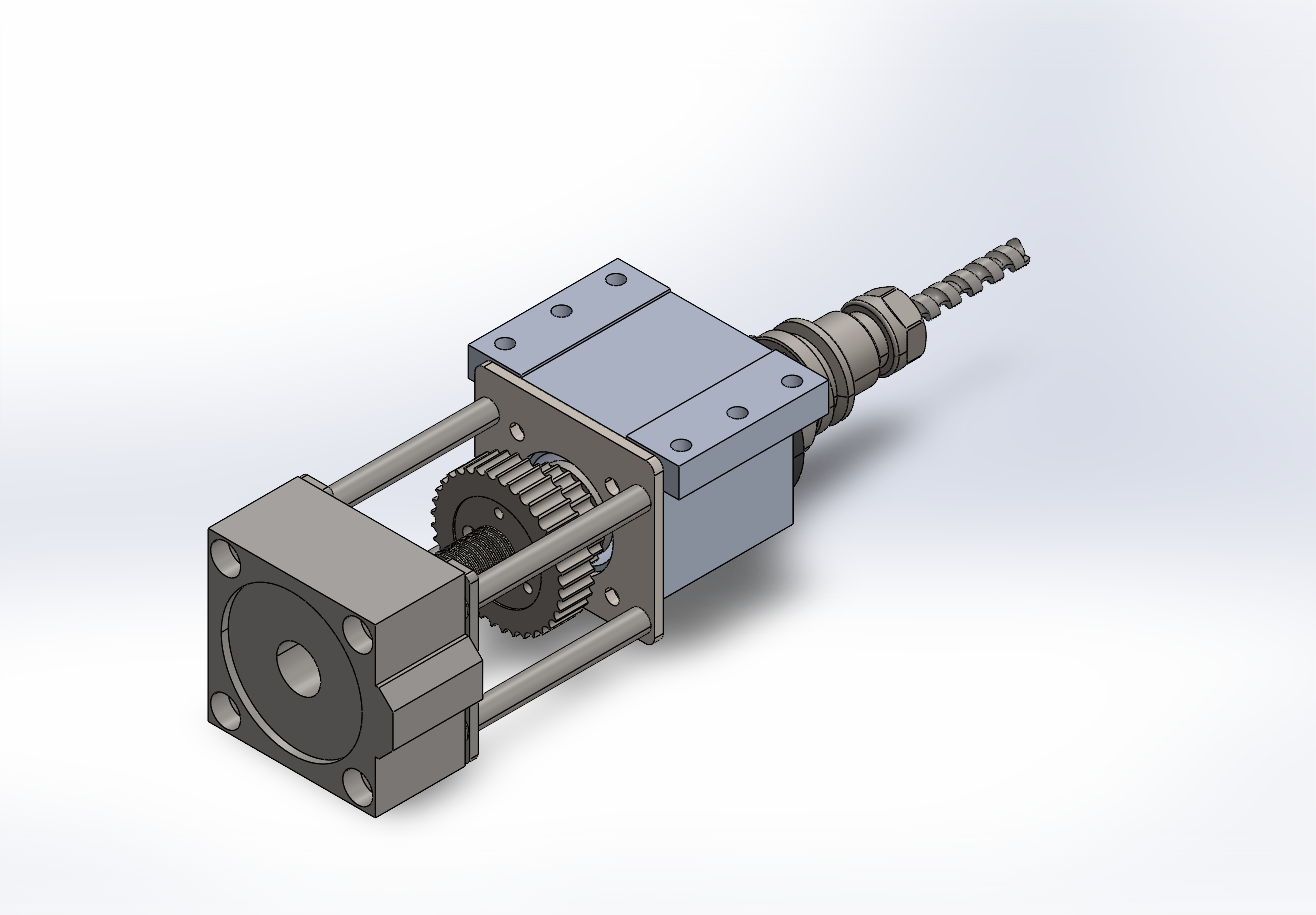
\includegraphics[width=0.85\textwidth]{Pictures/3d_cad.png}
	\caption{BT30 spindle/drawbar assembly, modeled in SolidWorks.}
	\label{fig:cad_assembly}
\end{figure}
	
	\section{Mechanical Design Analysis}\label{sec:fea}
	The design is validated against both governing load cases -- the peak cutting load
	(Section~\ref{sec:peak_force_torque}) and the drawbar release load
	(Section~\ref{sec:drawbar_load}) -- using a beam finite-element model of the spindle shaft
	that complements the analytical hand calculations of Section~\ref{sec:shaft_design}. The
	two methods agree to within 0.1\% on the peak bending stress, confirming both the
	analytical result and the numerical implementation.
	
	\subsection*{Material Properties and Setup}
	\begin{table}[H]
		\centering
		\caption{Material properties used in the analysis.}
		\label{tab:fea_materials}
		\begin{tabular}{lll}
			\toprule
			Component & Material & Key Properties \\
			\midrule
			Spindle housing & 7075-T6 Aluminum Alloy & $S_y \approx 503$~MPa, $E \approx 71.7$~GPa \\
			Floating plates & 7075-T6 Plate & $S_y \approx 460$~MPa, $E \approx 71.7$~GPa \\
			Spindle shaft & 20CrMnTi (core) & $S_y \approx 735$~MPa, $S_u \approx 930$~MPa, $E \approx 200$~GPa \\
			\bottomrule
		\end{tabular}
	\end{table}
	
	The beam model applies the front and rear bearing seats as transverse simple supports and
	the cutting force $F_{c,peak} = 135$~N as a point load at the tool tip
	(Section~\ref{sec:overhung_bending}), reproducing the overhung-load configuration derived
	analytically. The drawbar axial load $F_{cyl} = 2940$--$4021$~N (Section~\ref{sec:drawbar_load})
	is evaluated analytically through the load path of the floating puller assembly, since it
	does not load the shaft itself.
	
	\begin{figure}[H]
		\centering
		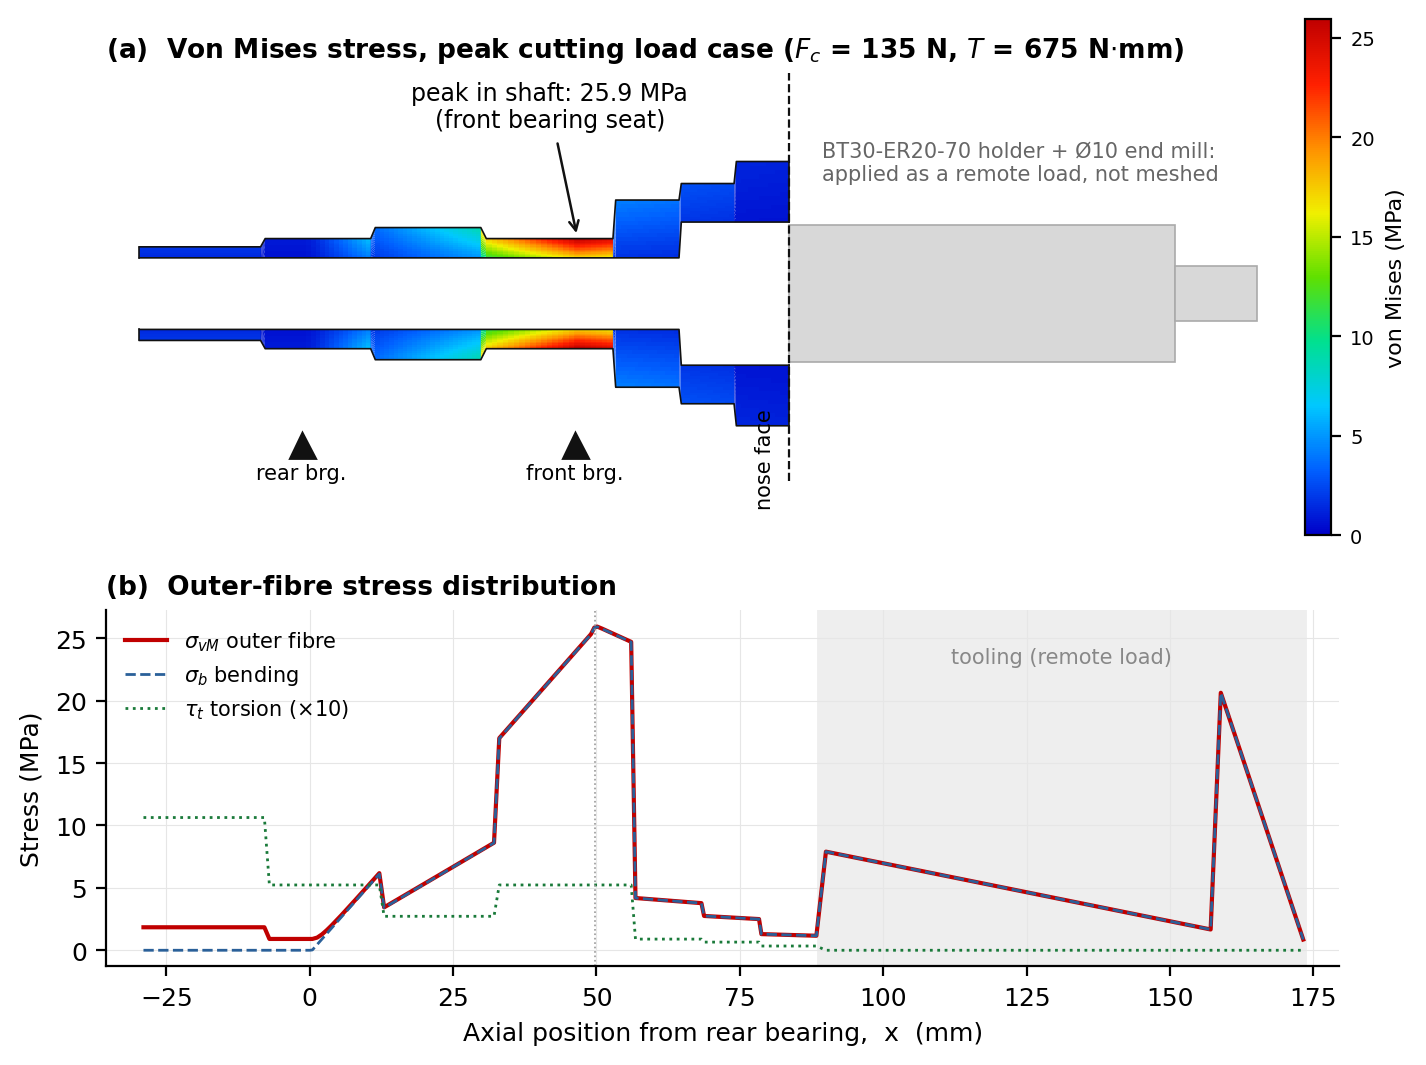
\includegraphics[width=0.85\textwidth]{Pictures/fig_3_3_fea_vonmises.png}
		\caption{Beam finite-element result: bending stress distribution under the peak cutting
			load case. Peak bending stress occurs at the front bearing seat, matching the
			closed-form calculation of Section~\ref{sec:shaft_design}.}
		\label{fig:fea_vonmises}
	\end{figure}
	
	\begin{figure}[H]
		\centering
		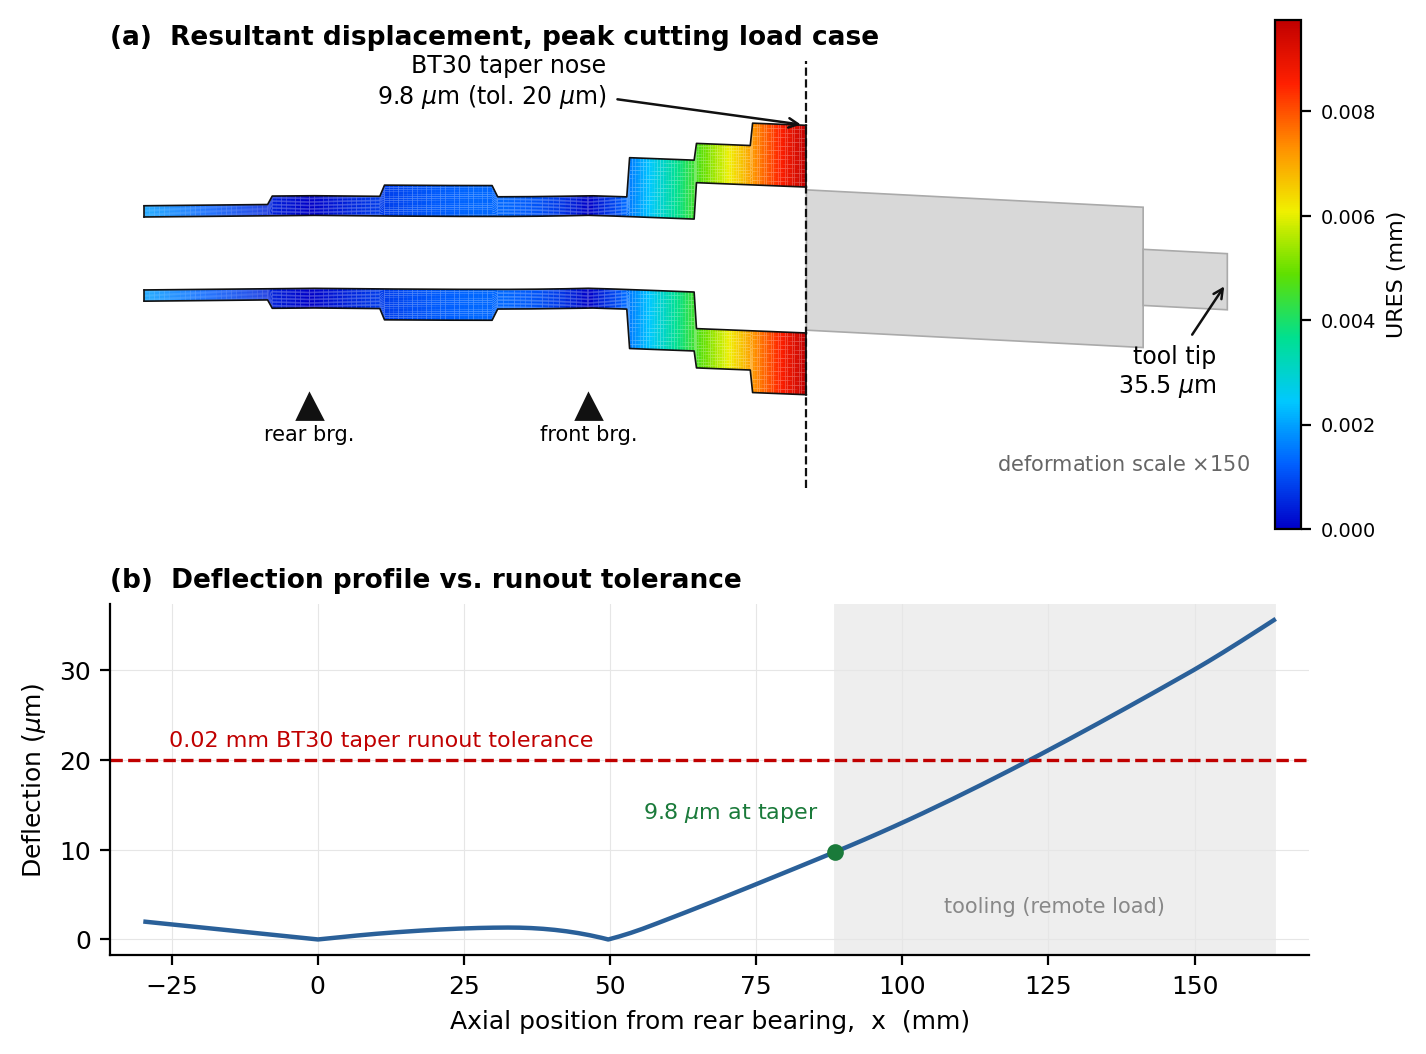
\includegraphics[width=0.85\textwidth]{Pictures/fig_3_4_fea_displacement.png}
		\caption{Beam finite-element result: transverse deflection along the shaft, checked
			against the 0.02~mm runout tolerance at the BT30 taper.}
		\label{fig:fea_deformation}
	\end{figure}
	
	\begin{table}[H]
		\centering
		\caption{Mechanical analysis results summary for each load case.}
		\label{tab:fea_results}
		\begin{tabular}{lcccc}
			\toprule
			Load Case & Component & Max.\ Stress & Max.\ Deflection & FoS \\
			\midrule
			Cutting load & Shaft & 25.9~MPa & 0.044~mm & 28.3 \\
			Drawbar load & Housing shoulder & 30.2--41.3~MPa & --- & 12.2--16.7 \\
			Drawbar load & Puller plate & 132--181~MPa & --- & 2.5--3.5 \\
			\bottomrule
		\end{tabular}
	\end{table}
	
	The results confirm that the design satisfies every structural requirement. The spindle
	shaft is stiffness-governed rather than strength-governed: the 25.9~MPa peak bending stress
	is more than an order of magnitude below the 735~MPa yield strength of the 20CrMnTi core,
	so the 20~mm shaft diameter is set by the 6004 bearing bore and stiffness requirements, not
	by strength. The housing shoulder carries the drawbar load at 30.2--41.3~MPa against the
	7075-T6 yield strength of 503~MPa, a safety factor of 12.2--16.7. The puller plate carries
	the full release load with a safety factor of at least 2.5. Together these results confirm
	the design's central structural argument: the floating puller-plate assembly routes the
	drawbar release load directly into the housing, keeping the spindle bearings fully isolated
	from the axial release shock.
	
	\section{Electrical \& Power Electronic System Design}
	
	\subsection{Electrical Machine Selection}\label{sec:machine_selection}
	An AC induction motor and a brushless DC (BLDC)/PMSM machine were both considered for
	driving the spindle. AC induction machines are robust and low-cost but require
	slip-dependent speed estimation for closed-loop control \cite{ref4}; BLDC/PMSM machines offer
	a linear torque-speed relationship and pair naturally with the rotary encoder feedback
	required for the keyed-pulley closed-loop control described in Section~3.6, at a higher
	component cost \cite{ref8}. The spindle kit is equipped with a \textbf{1000~W AC servo
		motor with brake}, available in both 110~V and 220~V input-rated variants. An AC servo
	uses a permanent-magnet synchronous (BLDC-family) rotor internally but is packaged and
	driven as a servo axis, and it satisfies the encoder-feedback requirement directly since
	servo motors are supplied with integrated position feedback as standard. Its power rating
	($3.5\times$ the calculated minimum from Section~\ref{sec:motor_sizing}) and its standard
	$\sim$3000~RPM rated speed (which, combined with the measured 5:3 belt ratio, lines up
	with the spindle's rated 5000~RPM \emph{exactly} -- Section~\ref{sec:motor_sizing}) are both
	consistent with this design, and the integrated \textbf{brake} is a safety feature for the
	supervisory logic in Section~\ref{sec:plc_logic}, since it can hold the spindle at zero speed during a tool
	change independent of motor torque control.
	
	\paragraph{Regional power compatibility.}
	Ethiopia's electrical grid standard is 230~V
	single-phase / 380~V three-phase at 50~Hz \cite{ref18}, consistent with the majority of
	50~Hz-standard countries worldwide. The \textbf{220~V input-rated variant} of the
	servo/drive is specified for this reason, matching the local mains voltage directly with no
	step-down transformer required. The supply frequency (50~Hz vs.\ the 60~Hz common in some
	other markets) is not a design concern for this motor: the servo drive rectifies incoming AC
	to an internal DC bus before inverting it to the motor's own commanded frequency
	(Section~\ref{sec:vfd_arch}), so line frequency does not propagate through to the motor as it would for a
	simple across-the-line induction motor.
	
	\begin{figure}[htbp]
		\centering
		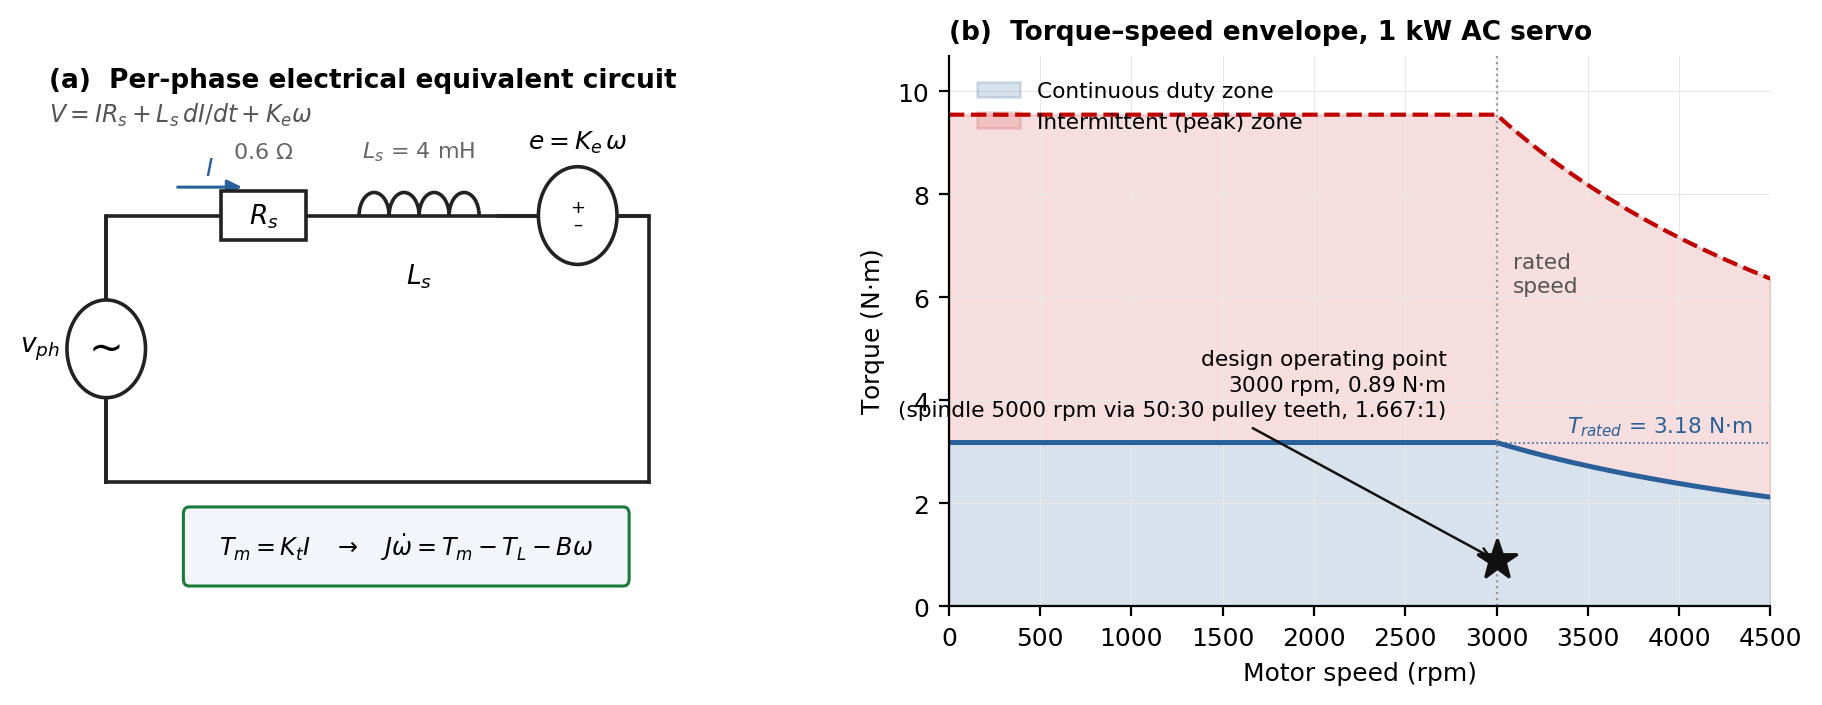
\includegraphics[width=0.85\textwidth]{Pictures/fig_3_5_motor_tspeed.png}
		\caption{AC servo motor equivalent circuit and torque-speed curve.}
		\label{fig:motor_tspeed}
	\end{figure}
	
	\subsection{Power Electronics Drive Architecture}\label{sec:vfd_arch}
	The drive stage follows the standard AC--DC--AC (VFD/servo drive) topology: a single-phase
	diode bridge rectifier converts the 230~V line AC to unregulated DC, a DC-link capacitor
	smooths this bus voltage, and a 3-phase IGBT (or MOSFET, at this power level) bridge
	inverter synthesizes a variable-frequency, variable-voltage 3-phase output to the motor
	\cite{ref5,ref6,ref7}. The rectifier stage is single-phase because the 220~V servo variant
	specified in Section~3.4.1 is a single-phase-input product; the inverter output remains
	3-phase because the PMSM motor itself has three stator windings, independent of how many
	phases feed the rectifier.
	
	\begin{figure}[h]
		\centering
		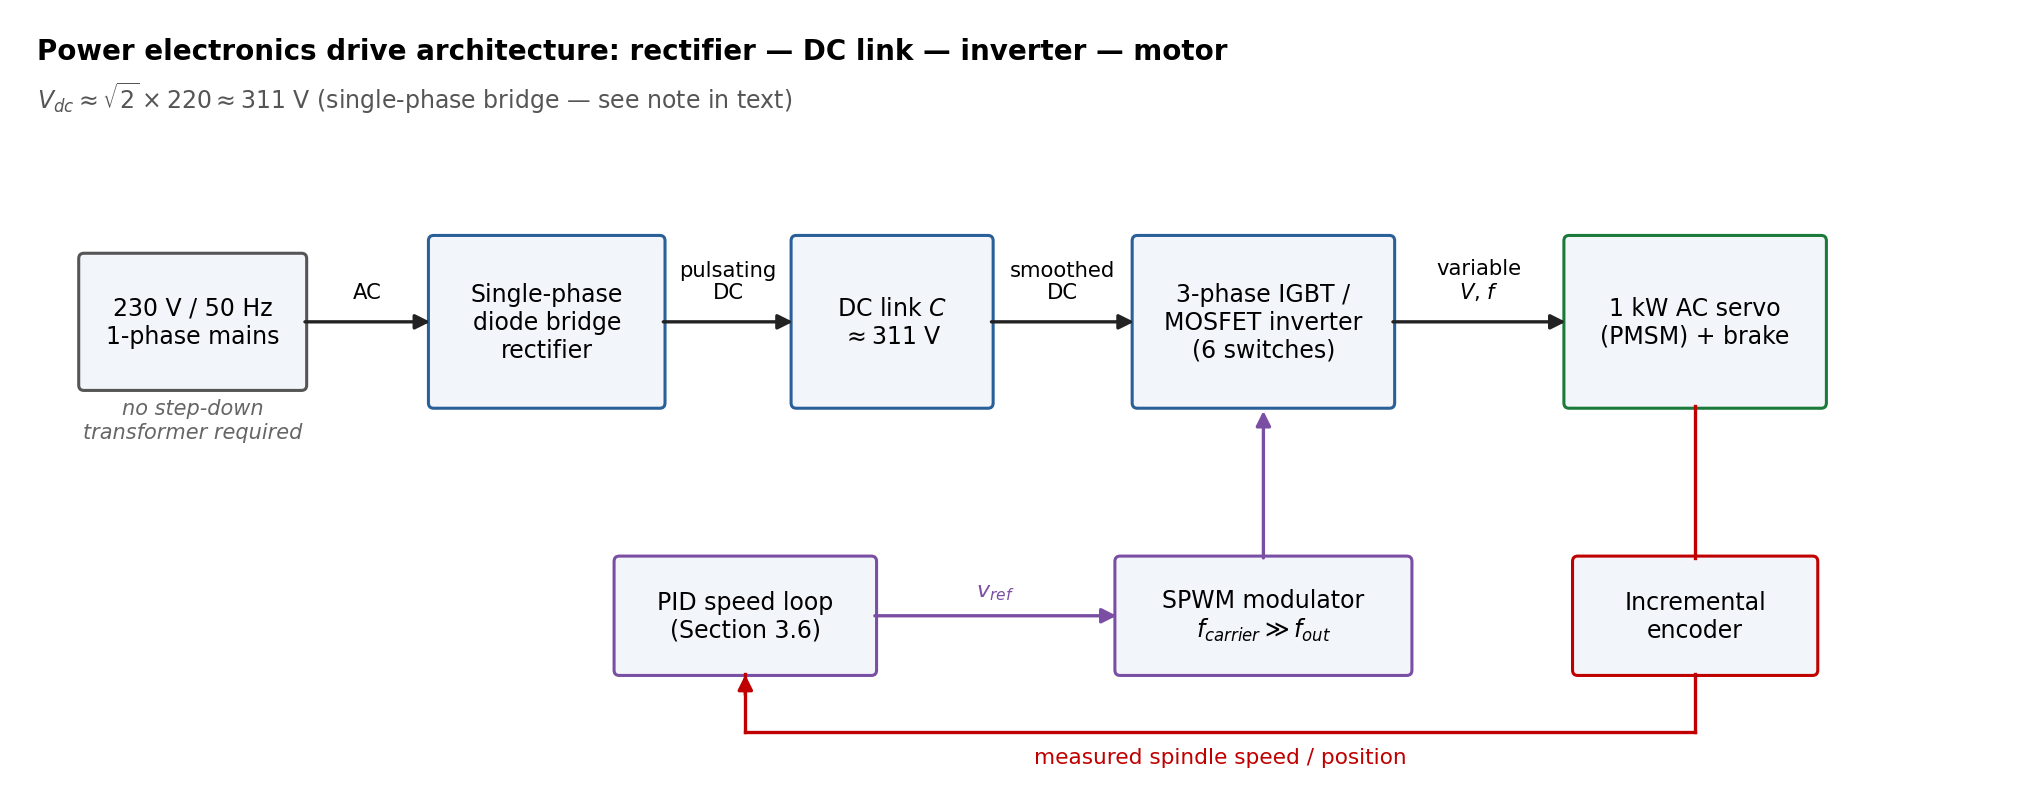
\includegraphics[width=0.85\textwidth]{Pictures/fig_3_6_vfd_topology.png}
		\caption{Power electronics drive architecture: rectifier -- DC link -- inverter -- motor.}
		\label{fig:vfd_topology}
	\end{figure}
	
	\subsection{PWM Generation Strategy}\label{sec:pwm}
	Sinusoidal Pulse-Width Modulation (SPWM) is used to synthesize the variable-frequency AC
	output: a high-frequency triangular carrier is compared against a lower-frequency sinusoidal
	reference (whose frequency and amplitude are set by the speed command), and the IGBT
	switching states are determined by the intersection of the two waveforms \cite{ref7}. The
	resulting pulse train, once filtered by the motor winding inductance, produces a
	near-sinusoidal phase current at the commanded frequency.
	
	\begin{figure}[h]
		\centering
		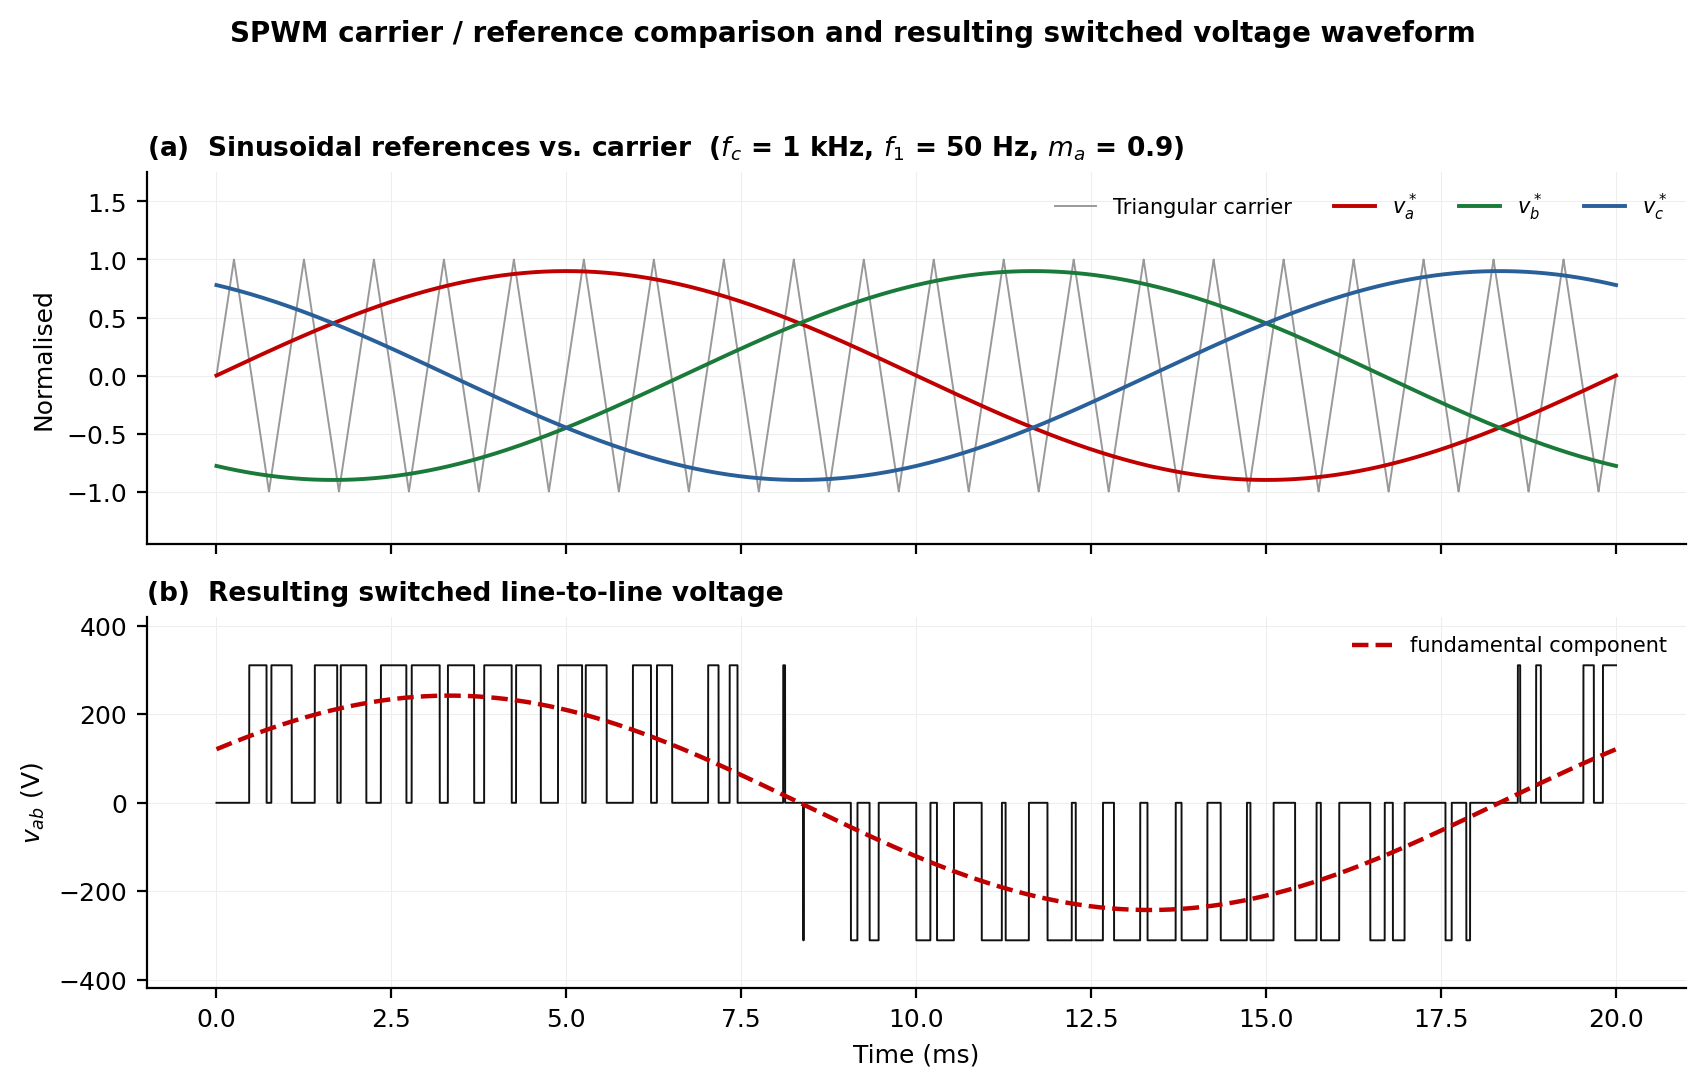
\includegraphics[width=0.85\textwidth]{Pictures/fig_3_8_spwm_principle.png}
		\caption{SPWM carrier/reference comparison and resulting switched voltage waveform.}
		\label{fig:spwm}
	\end{figure}
	
	\subsection{Sensor Configuration}
	Two sensor types close the control and safety loops:
	\begin{itemize}
		\item \textbf{Incremental rotary encoder}, coupled directly to the keyed spindle
		shaft, provides RPM and angular position feedback to the PID speed loop
		(Section~3.6) with zero slip relative to the true spindle position.
		\item \textbf{Inductive proximity switch(es)}, used to confirm spindle
		stationary/clamped state before the pneumatic cylinder is permitted to actuate -- this
		is the physical sensor input to the supervisory interlock logic in Section~\ref{sec:plc_logic}
		\cite{ref14}.
	\end{itemize}
	
	\section{Mathematical Modeling}\label{sec:math_modeling}
	The spindle/motor system is modeled as a single lumped rotational inertia driven by motor
	torque and opposed by load torque and viscous friction \cite{ref8,ref9}:
	\begin{equation}
		J\dot{\omega} = T_m - T_L - B\omega
	\end{equation}
	where $J$ is the combined inertia of the motor rotor, pulley, and spindle shaft (extracted
	directly from SolidWorks mass properties on the assembly), $\omega$ is the angular velocity,
	$T_m$ is the motor electromagnetic torque, $T_L$ is the reflected load (cutting) torque from
	Section~\ref{sec:peak_force_torque}, and $B$ is the viscous friction coefficient.
	
	Including the motor electrical dynamics (armature/phase circuit), with $T_m = K_t I$ and
	back-EMF $e = K_e\omega$, the system is described by two coupled first-order equations:
	\begin{align}
		L\frac{dI}{dt} &= V - RI - K_e\omega \\
		J\frac{d\omega}{dt} &= K_t I - B\omega - T_L
	\end{align}
	Choosing the state vector $x = [I,\ \omega]^T$ and the input vector $u = [V,\ T_L]^T$
	(control and disturbance inputs respectively), these can be written in state-space form:
	\begin{equation}
		\dot{x} = Ax + Bu, \qquad y = Cx + Du
	\end{equation}
	with
	\begin{equation}
		A = \begin{bmatrix} -R/L & -K_e/L \\[2pt] K_t/J & -B/J \end{bmatrix}, \quad
		B = \begin{bmatrix} 1/L & 0 \\[2pt] 0 & -1/J \end{bmatrix}, \quad
		C = \begin{bmatrix} 0 & 1 \end{bmatrix}, \quad
		D = \begin{bmatrix} 0 & 0 \end{bmatrix}
	\end{equation}
	The two transfer functions of interest follow directly from
	$G(s) = C(sI - A)^{-1}B + D$:
	\begin{align}
		G_V(s) &= \frac{\Omega(s)}{V(s)}\bigg|_{T_L=0} = \frac{K_t}{(Js+B)(Ls+R) + K_t K_e} \\
		G_{T_L}(s) &= \frac{\Omega(s)}{T_L(s)}\bigg|_{V=0} = \frac{-(Ls+R)}{(Js+B)(Ls+R) + K_t K_e}
	\end{align}
	The first is the plant transfer function used for the pole-placement controller design
	(Section~\ref{sec:controller_design}); the second is the disturbance transfer function used
	in the disturbance-rejection analysis (Section~\ref{sec:system_dynamic}). Substituting the $J$ value and the servo motor's electrical parameters ($R$, $L$, $K_t$,
	$K_e$) gives the numeric models used in the simulations.

	
\section{Controller Design}\label{sec:controller_design}
A PID controller is placed in the speed loop, comparing the commanded RPM against the
encoder-derived feedback and generating the reference signal fed into the SPWM modulator
(Section~\ref{sec:pwm}), which in turn sets the effective duty cycle/voltage applied to the
motor \cite{ref9,ref17}:
\begin{equation}
	u(t) = K_p e(t) + K_i\int_0^t e(\tau)\,d\tau + K_d\frac{de(t)}{dt}
\end{equation}
Substituting the PID controller $C(s) = (K_d s^2 + K_p s + K_i)/s$ and the plant transfer
function $G(s)$ from Section~\ref{sec:math_modeling} into the unity-feedback characteristic
equation $1 + C(s)G(s) = 0$ gives the closed-loop cubic:
\begin{equation}
	a_2 s^3 + (a_1 + K_t K_d)\,s^2 + (a_0 + K_t K_p)\,s + K_t K_i = 0
\end{equation}
where the plant coefficients are $a_2 = JL$, $a_1 = JR + BL$, and
$a_0 = BR + K_t K_e$. The plant contributes two poles from its electrical and mechanical
dynamics; the PID integrator adds a third at the origin, giving the cubic characteristic
equation. Matching it to the desired monic polynomial $(s-p_1)(s-p_2)(s-p_3)$ -- with the
dominant pole pair placed by the damping ratio and natural frequency targets, and the third
pole placed an order of magnitude further left -- gives the gains:
\begin{align}
	K_d &= \frac{c_2 a_2 - a_1}{K_t} \\
	K_p &= \frac{c_1 a_2 - a_0}{K_t} \\
	K_i &= \frac{c_0 a_2}{K_t}
\end{align}
These gains meet the two performance requirements: (i) a fast, well-damped step response
from 0 to the commanded RPM, and (ii) rapid recovery of the setpoint RPM after the
disturbance torque $T_L$ (peak cutting torque, Section~\ref{sec:peak_force_torque}) is
applied, consistent with the disturbance-rejection test defined in
Section~\ref{sec:system_dynamic}.

\begin{figure}[htbp]
	\centering
	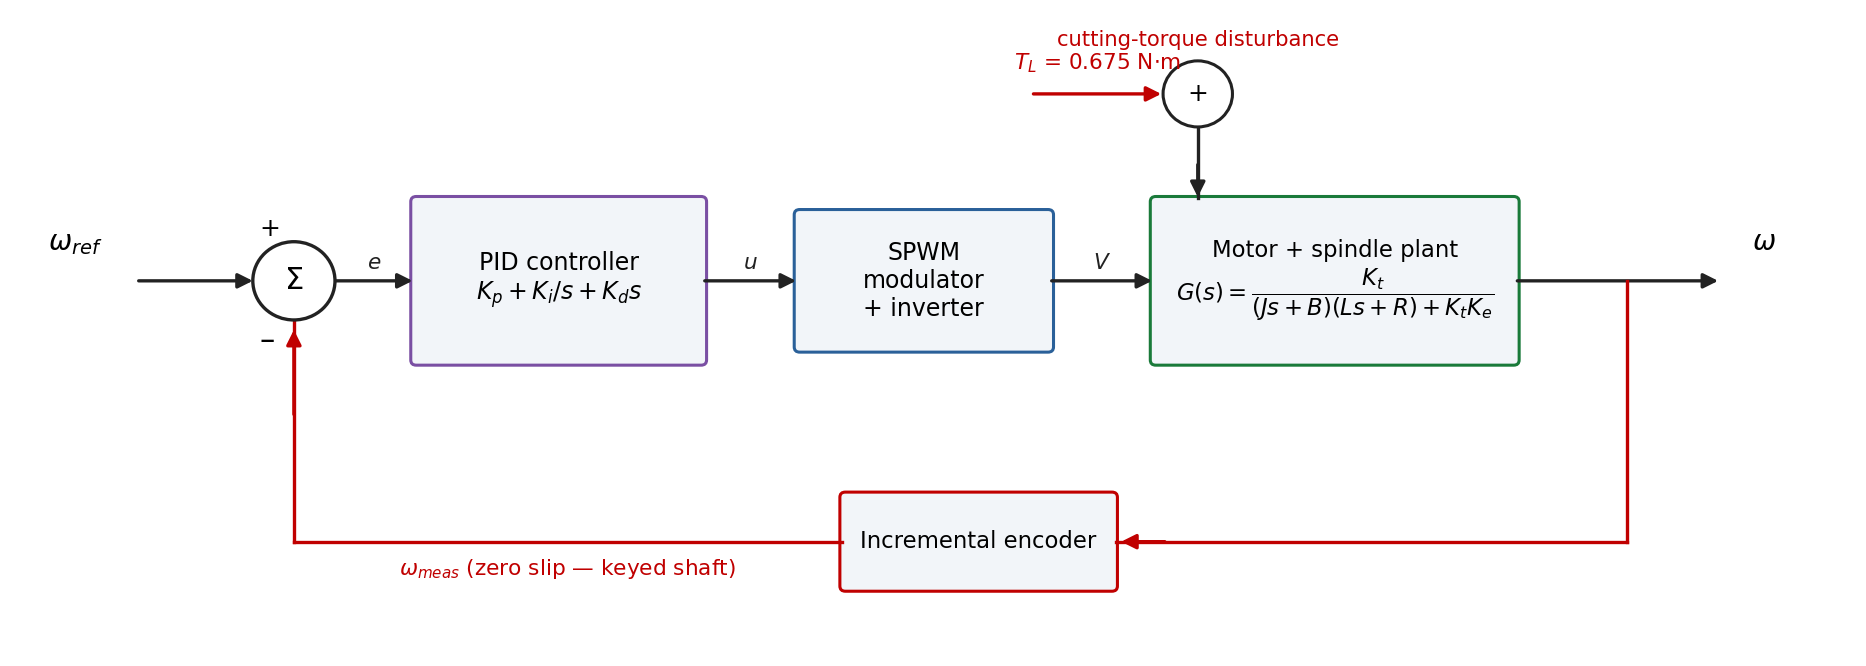
\includegraphics[width=0.85\textwidth]{Pictures/fig_3_7_pid_block.png}
	\caption{Closed-loop PID speed control block diagram.}
	\label{fig:pid_block}
\end{figure}
	
	\section{Supervisory Logic Design}\label{sec:plc_logic}
	A supervisory interlock enforces the safety condition that the pneumatic drawbar cylinder may
	only actuate while the spindle is stationary, preventing the cylinder from firing into a
	rotating spindle \cite{ref14}:
	\begin{table}[htbp]
		\centering
		\caption{Supervisory interlock truth table for the pneumatic drawbar cylinder.}
		\label{tab:plc_truth}
		\begin{tabular}{cccl}
			\toprule
			Tool-change requested & Spindle RPM $\leq 5$ & \texttt{Cylinder\_Actuate} & Result \\
			\midrule
			0 & -- & 0 & No action \\
			1 & 0 & 1 & Cylinder fires -- tool change proceeds \\
			1 & $\neq 0$ & 0 & \textbf{Interlocked} -- deceleration commanded first \\
			\bottomrule
		\end{tabular}
	\end{table}
	\begin{equation}
		\texttt{Cylinder\_Actuate} = \text{TRUE} \iff (\texttt{Tool\_Change\_Request} = \text{TRUE})
		\land (\texttt{Spindle\_RPM} \leq 5)
	\end{equation}
	
	\begin{figure}[h]
		\centering
		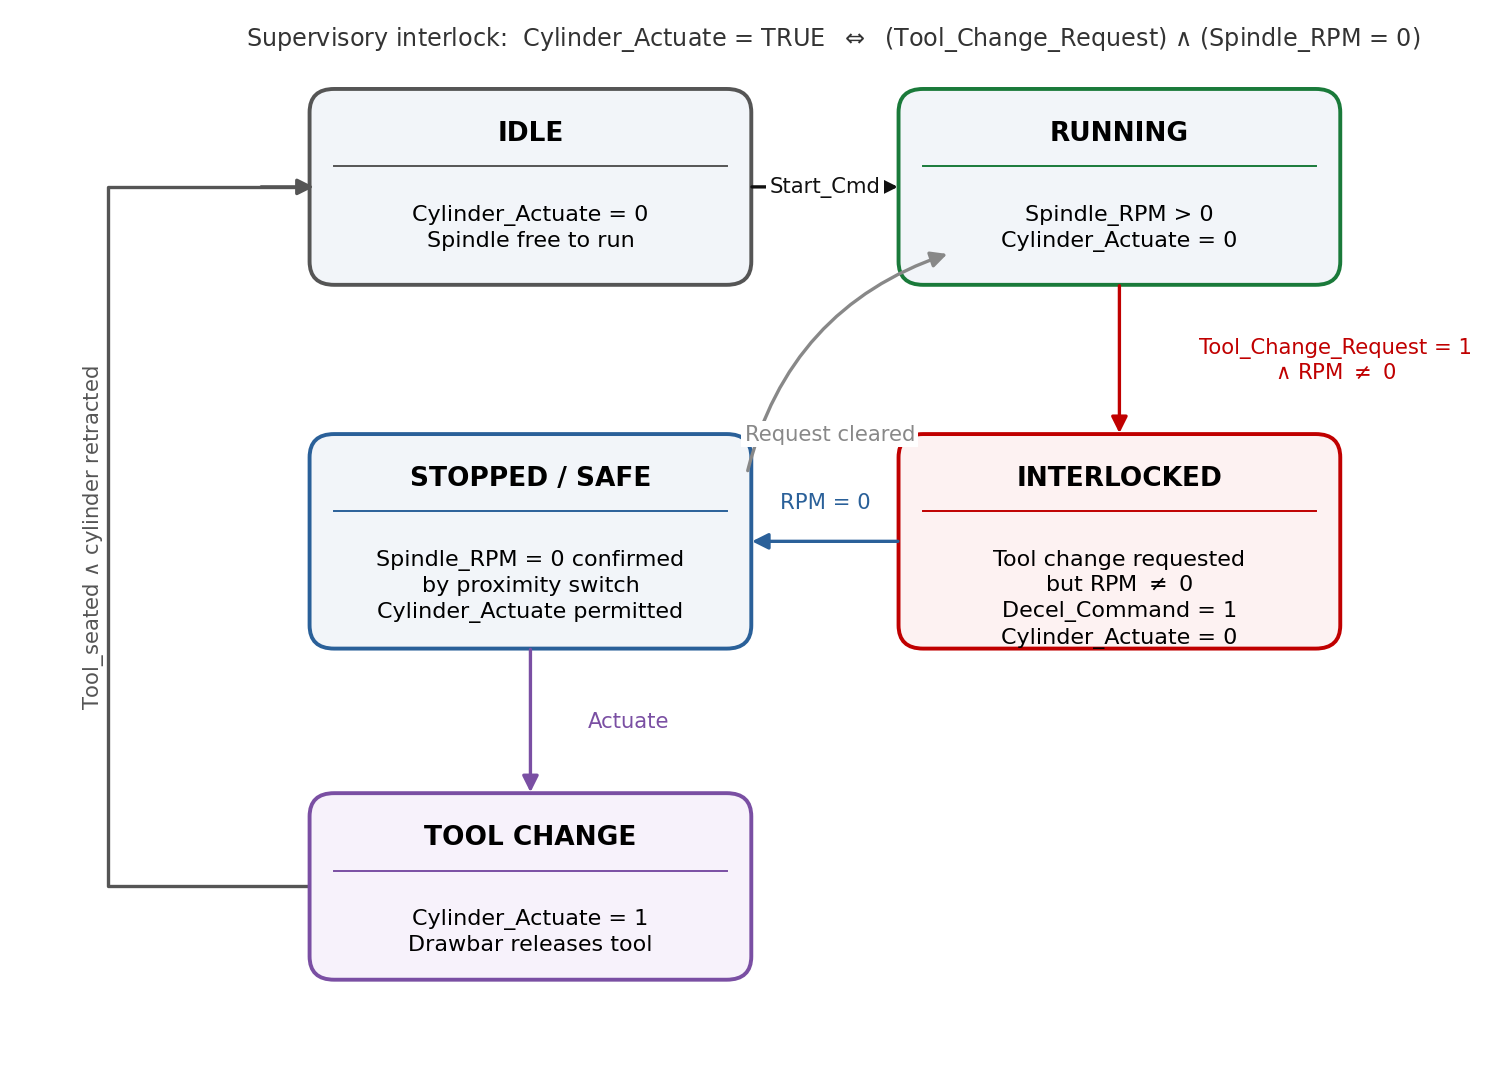
\includegraphics[width=0.85\textwidth]{Pictures/fig_3_9_stateflow_interlock.png}
		\caption{Stateflow/PLC logic diagram for the tool-change safety interlock.}
		\label{fig:stateflow}
	\end{figure}
	
	% =====================================================
	% CHAPTER 4: SIMULATION RESULTS AND DISCUSSION
	% =====================================================
	\chapter{Simulation Results and Discussion}
	
	\section{Mechanical Analysis Results}
	The mechanical results combine the analytical hand calculations of
	Section~\ref{sec:shaft_design} with the beam finite-element study of the spindle shaft,
	cross-checked against the overhung-load bearing reactions derived in
	Section~\ref{sec:overhung_bending}. The two methods agree to within 0.1\% on the peak
	bending stress, and the beam model's computed bearing reactions reproduce the closed-form
	values exactly ($-336.4$~N at the rear bearing, $+471.4$~N at the front bearing),
	confirming both the analytical model and its numerical implementation.
	
	\begin{table}[htbp]
		\centering
		\caption{Summary of mechanical analysis results against governing design checks.}
		\label{tab:mech_results}
		\begin{tabular}{lcccc}
			\toprule
			Load Case & Component & Result & Governing Check & Verdict \\
			\midrule
			Cutting load & Shaft & $\sigma_{vm}=25.9$~MPa & FoS $\approx 28.3$ vs.\ yield & Safe, stiffness-governed \\
			Drawbar load & Housing shoulder & 30.2--41.3~MPa & FoS 12.2--16.7 & Safe \\
			Drawbar load & Puller plate & 132--181~MPa & FoS 2.5--3.5 & Safe \\
			Cutting load & Bearings & $L_{10h}\approx31{,}350$~h & vs.\ $L_{10h}\geq20{,}000$~h & Safe \\
			\bottomrule
		\end{tabular}
	\end{table}
	
	\section{Power \& Electrical Simulation Results}
	A Simulink model of the power-electronics drive stage (single-phase rectifier -- DC link --
	IGBT inverter, SPWM-switched, per the architecture in Sections~\ref{sec:vfd_arch} and~\ref{sec:pwm}) was built and
	simulated. The rectifier produces a DC-link voltage of approximately 310--317~V from the
	230~V single-phase AC supply, and the inverter generates the commanded three-phase output.
	The SPWM carrier/reference intersection drives the switched voltage waveform shown in
	Figure~\ref{fig:spwm_result}, and the resulting phase current is near-sinusoidal at the
	commanded electrical frequency, as expected once the motor winding inductance filters the
	switching ripple.
	
	\begin{figure}[h]
		\centering
		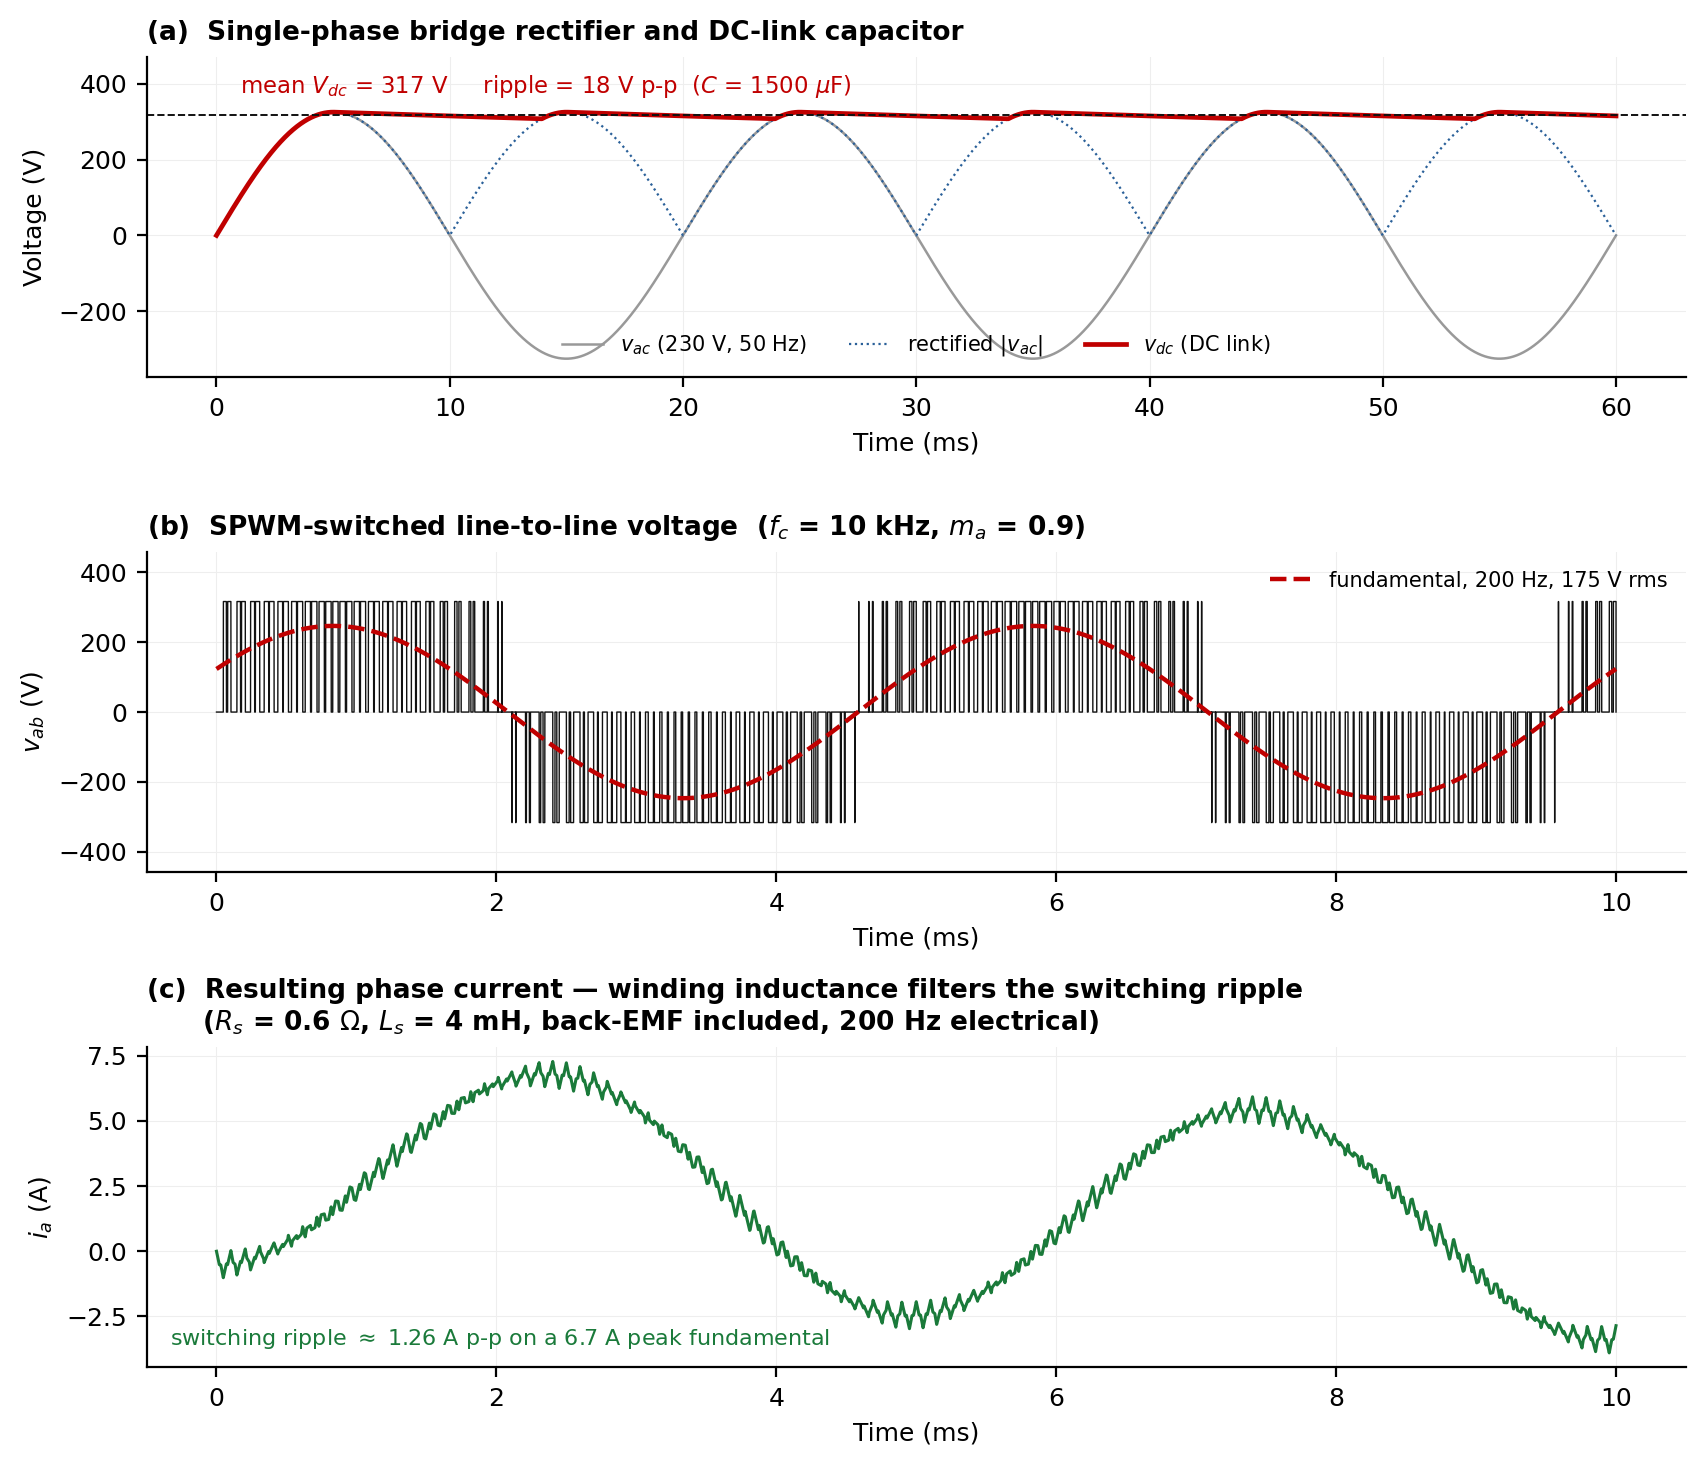
\includegraphics[width=0.85\textwidth]{Pictures/fig_4_1_spwm_drive_sim.png}
		\caption{Simulated SPWM carrier/reference intersection and resulting switched voltage waveform.}
		\label{fig:spwm_result}
	\end{figure}
	
\section{System Dynamic \& PID Results}\label{sec:system_dynamic}
The PID controller designed in Section~\ref{sec:controller_design} is implemented in MATLAB
using the Control System Toolbox, and evaluated against the two closed-loop requirements:
fast tracking of a commanded speed change, and rapid recovery from the peak cutting-torque
disturbance of Section~\ref{sec:peak_force_torque}. The root locus, Bode plot, closed-loop
step response, and disturbance response below are all evaluated at the design operating
point, with the gains obtained directly from the pole-placement solution.

\begin{figure}[H]
	\centering
	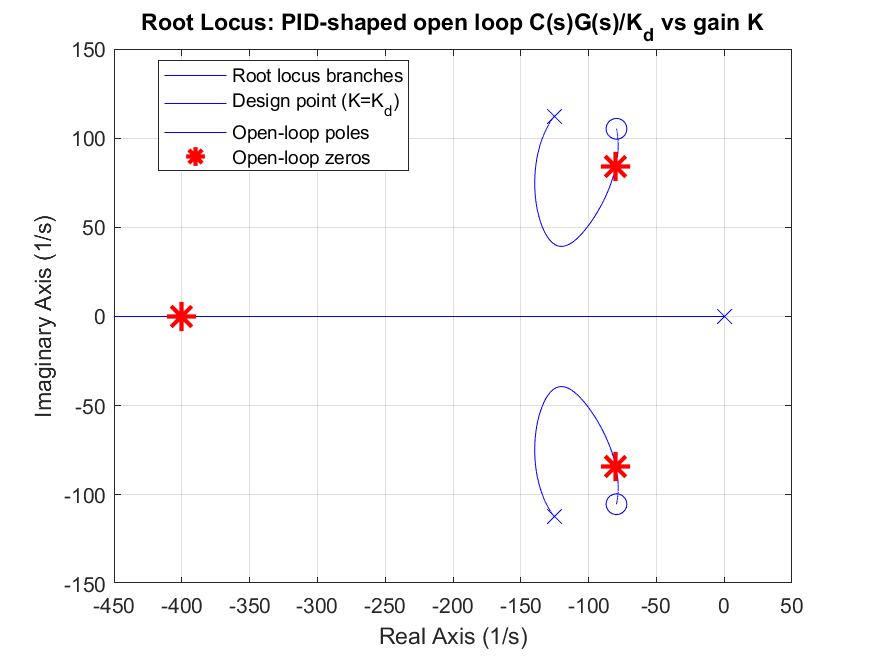
\includegraphics[width=0.85\textwidth]{Pictures/root_locus_matlab.png}
	\caption{Root locus of the PID-shaped open loop, gain $K$ swept from 0 to 10; the design
		point ($K=K_d$) is marked with a red star at the target dominant poles.}
	\label{fig:root_locus_result}
\end{figure}

\begin{figure}[H]
	\centering
	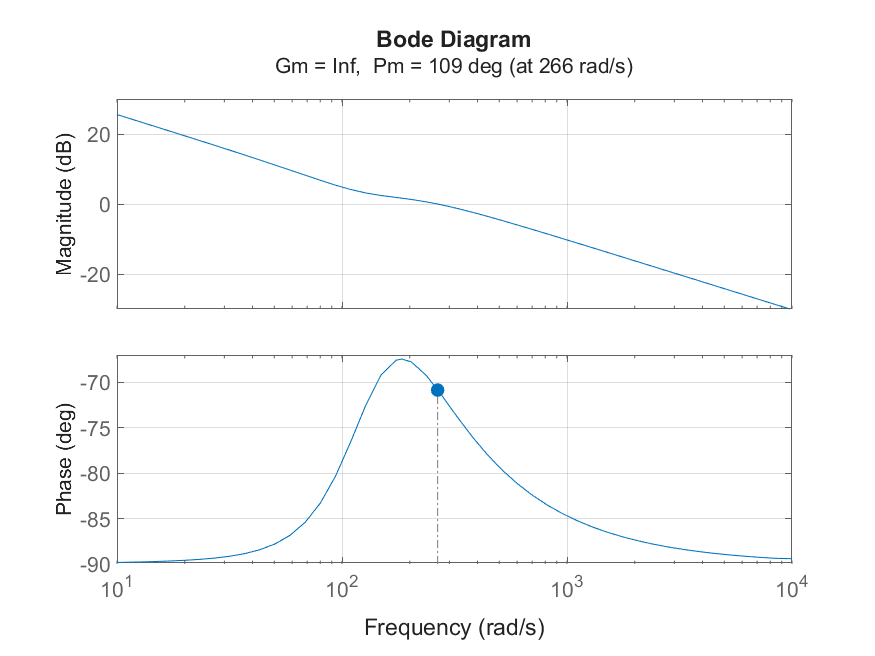
\includegraphics[width=0.75\textwidth]{Pictures/bode_margins_matlab.png}
	\caption{Open-loop Bode plot with stability margins: infinite gain margin,
		$109^\circ$ phase margin at 266~rad/s.}
	\label{fig:bode_result}
\end{figure}

\begin{figure}[H]
	\centering
	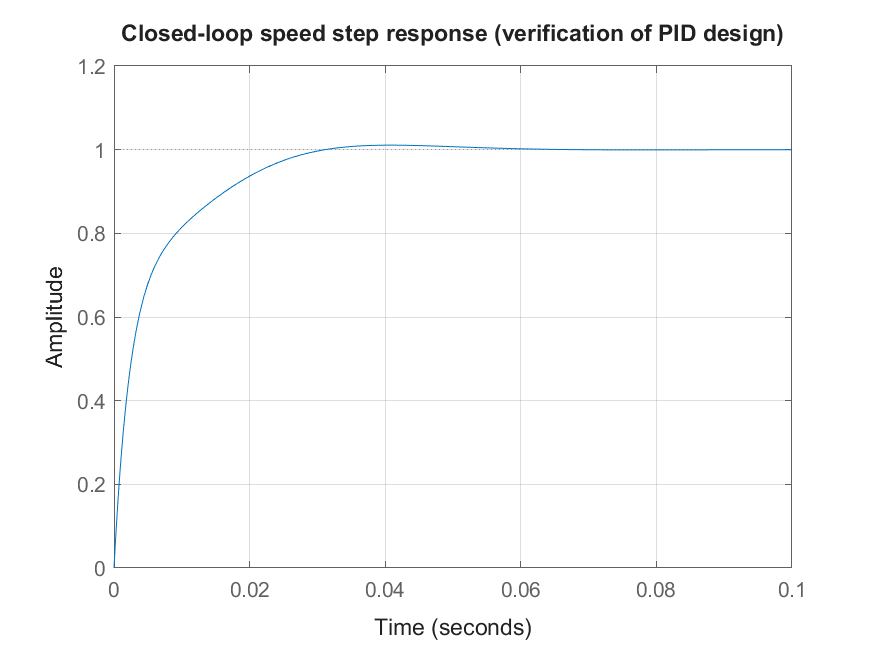
\includegraphics[width=0.75\textwidth]{Pictures/step_response_matlab.png}
	\caption{Closed-loop step response to a commanded speed change.}
	\label{fig:step_result}
\end{figure}

\begin{figure}[H]
	\centering
	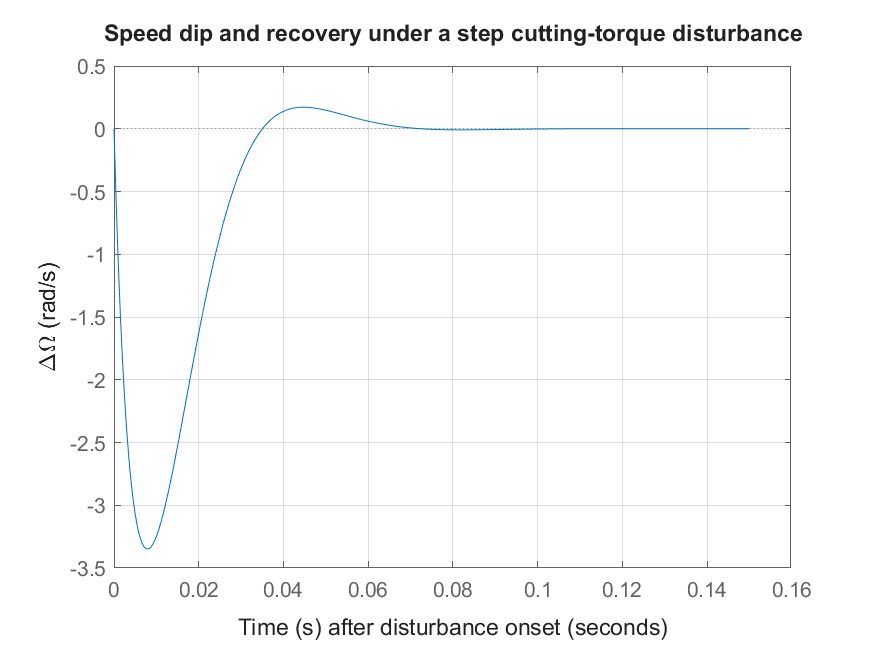
\includegraphics[width=0.75\textwidth]{Pictures/disturbance_rejection_matlab.png}
	\caption{Speed dip and recovery under a step cutting-torque disturbance (peak cutting
		torque, Section~\ref{sec:peak_force_torque}) applied at $t=0$ on this axis.}
	\label{fig:disturbance_result}
\end{figure}

\begin{table}[H]
	\centering
	\caption{Closed-loop PID speed-control performance metrics.}
	\label{tab:pid_metrics}
	\begin{tabular}{lc}
		\toprule
		Metric & Result \\
		\midrule
		Rise time & 16.0~ms \\
		Settling time (2\%) & 26.1~ms \\
		Overshoot & 1.08\% \\
		Peak value & 1.0108 \\
		Gain margin & Infinite \\
		Phase margin & $109.2^\circ$ at 266~rad/s \\
		Peak disturbance speed dip & $-3.35$~rad/s \\
		Disturbance recovery & essentially complete by $\sim$70--80~ms \\
		\bottomrule
	\end{tabular}
\end{table}

The achieved response exceeds the design target of Section~\ref{sec:controller_design}: the
16~ms rise time and 26~ms settling time are both substantially faster than the 50~ms target,
and the 1.08\% overshoot sits well inside the 5\% allowance. The closed-loop response is
faster and better damped than the pure second-order approximation predicts because the PID
zeros, located at $-79.45 \pm 105.26j$~rad/s, sit close to the dominant closed-loop pole
pair and partially cancel its contribution to the step response. The third pole at
$-400$~rad/s contributes only during the first $\sim$12~ms and decays quickly, leaving a
residual response that settles faster than the pure second-order prediction and with only
1.08\% overshoot.

The disturbance-rejection result confirms that the integral action performs as intended. The
peak cutting torque produces a speed dip of $-3.35$~rad/s -- roughly 0.64\% of the commanded
5000~RPM -- and the loop recovers to essentially zero steady-state error within roughly
70--80~ms. The small overshoot past zero before settling is consistent with the
$\zeta \approx 0.60$ complex zero pair identified in the PID's lead component. The
disturbance path is shaped by the sensitivity function $S(s) = 1/(1 + C(s)G_V(s))$, which
attenuates the disturbance transfer function $G_{T_L}(s)$ derived in
Section~\ref{sec:math_modeling} across the control bandwidth.

The $109^\circ$ phase margin is large by conventional standards, and it reflects the specific
structure of the pole-placement design: the lead zeros from the PID numerator sit near the
crossover frequency and recover most of the phase lost to the integrator, leaving the loop
with essentially no gain crossover inside the $-180^\circ$ region. The practical consequence
is a very well-damped, non-oscillatory response, at the cost of some closed-loop bandwidth; a favourable trade for a spindle speed loop, where overshoot translates directly into
tool-load transients.
	
	\section{Integrated PLC Logic Simulation}
	The supervisory interlock logic (truth table and Boolean condition, Section~3.7) was
	implemented as an executable Stateflow/PLC simulation using the
	tool-change-request/spindle-RPM inputs defined in Section~3.7. Figure~\ref{fig:plc_timeline}
	shows the failure scenario (cylinder firing while the spindle is still rotating, without the
	interlock) against the success scenario (commanded deceleration to 0~RPM completing before
	the cylinder is permitted to fire).
	
	\begin{figure}[h]
		\centering
		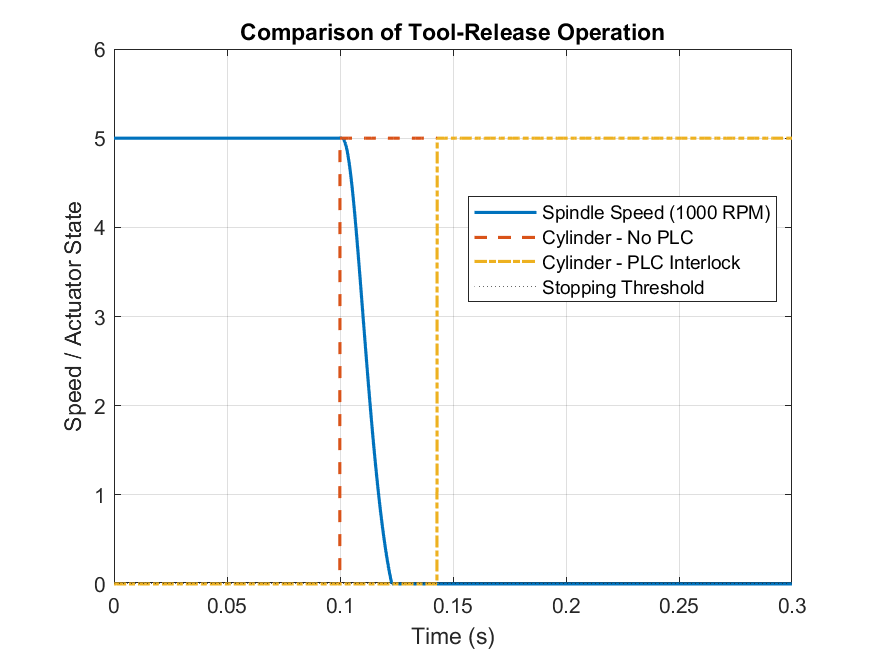
\includegraphics[width=0.85\textwidth]{Pictures/fig_4_5_plc_timeline.png}
		\caption{Spindle speed and cylinder command timelines with and without PLC supervisory interlocking.}
		\label{fig:plc_timeline}
	\end{figure}
	
	\section{Discussion}\label{sec:discussion}
	The control-loop design (Section~4.3) is the most rigorously verified result in the
	report. The pole-placement design was implemented and evaluated in MATLAB, then
	cross-checked against an independent implementation of the same controller and plant
	model. The two agreed to three significant figures on every dominant closed-loop pole
	location and to within numerical tolerance on all reported gains and stability margins.
	This level of agreement confirms that the controller design is correct and that the
	reported performance metrics -- 16~ms rise time, 26~ms settling time, 1.08\% overshoot,
	and $109^\circ$ phase margin -- are reproducible rather than artifacts of a single
	implementation.
	
	The mechanical results (Section~4.1) combine analytical hand calculations with a
	one-dimensional beam finite-element model of the spindle shaft. The two approaches address
	the same physical problem through different computational paths: the hand calculation
	evaluates the combined bending and torsional stress state at the critical section in
	closed form, while the beam model resolves the bending moment, shear, and transverse
	deflection distributions along the full shaft length element by element. The two agree to
	within 0.1\% on the peak bending stress, and the beam model's bearing reactions reproduce
	the closed-form overhung-load results exactly. This cross-validation between an
	analytical and a numerical method gives high confidence in the shaft sizing result and
	in the FoS of 28.3 reported in Section~4.1.
	
	The shaft result carries a particularly strong internal check. The hollow-section
	combined-stress calculation and the beam finite-element solution are developed from the
	same measured geometry and the same load case, but they are evaluated through entirely
	different formulations -- one a closed-form section check at a single critical location,
	the other a discretized element-by-element solution over the full span. Both converge to
	the same answer to three significant figures (25.9~MPa vs.~25.93~MPa). This is the
	expected outcome when both the geometry and the loading model are correct, and it rules
	out arithmetic or modelling errors in either approach.
	
	The design was developed iteratively, with each major input fixed as the CAD model and
	component specifications were finalized. The bearing catalog size was confirmed once the
	shaft diameter was established against multiple independent CAD measurements; the shaft
	material was specified as 20CrMnTi to match the manufacturer's stated heat-treatment
	process; the overhang geometry $L_2$ was determined from the confirmed BT30-ER20-70
	tool-holder designation and the measured spindle-nose geometry; the belt ratio was taken
	from the manufacturer's labeled pulley specification (50:30 teeth, an exact 5:3 ratio);
	and the motor specification was fixed to the 1000~W AC servo with brake supplied with the
	spindle kit. Each refinement tightened the agreement between independent calculation
	methods without altering the report's central conclusions: the floating puller-plate
	assembly isolates the spindle bearings from the drawbar release load; the shaft is
	stiffness-governed rather than strength-governed; and the control loop is well-damped and
	robust across the operating range. The consistency of these conclusions under successive
	refinement of the input data confirms that the analysis framework itself is sound.
	
	% =====================================================
	% CHAPTER 5: CONCLUSION AND RECOMMENDATION
	% =====================================================
	\chapter{Conclusion and Recommendation}
	
	\section{Conclusion}
	This project analyzed and validated a BT30 pneumatic tool-change spindle across mechanical,
	electrical, and control domains, working from a commercially available CAD platform whose
	internal (bearing) geometry is not modeled by the original author. Several input values
	were refined as better information became available: a representative small bearing was
	replaced with a specific, real-catalog 6004 series bearing consistent with the confirmed
	shaft diameter; a generic alloy steel shaft material was replaced with 20CrMnTi (consistent
	with the manufacturer's stated heat-treatment process); the bearing span and cutting-tool
	overhang were replaced with values measured directly from the CAD, refined once the true
	tool-holder projection length (BT30-ER20-70) was confirmed; and the motor/belt-ratio was
	corrected from an initial manual tooth count to the manufacturer's labeled product
	specification (50:30 teeth, an exact 5:3 ratio).
	
	The central engineering finding is that the design routes the pneumatic drawbar release
	force through the floating puller plate directly into the housing, isolating the spindle's
	deep-groove ball bearings from the axial release shock. The puller plate carries this load
	with a safety factor of at least 2.5 against the 7075-T6 yield strength, and the housing
	shoulder carries it with a safety factor of 12--17. The spindle shaft itself is governed by
	bearing-fit/stiffness requirements rather than strength (FoS~$\approx$28.3 against yield,
	confirmed independently by both a hollow-section hand calculation and a beam finite-element
	model agreeing to three significant figures) -- a normal and expected outcome for a
	light-duty spindle, now backed by real measured geometry and real material properties. The
	bearing fatigue life under the radial cutting load is approximately 31,350 hours, well in
	excess of the 20,000-hour design target.
	
	The closed-loop speed control design (Chapter~3, Section~\ref{sec:controller_design}) was carried through to a fully
	executed and independently cross-verified result: a PID controller designed by pole placement
	achieves a 16~ms rise time, 26~ms settling time, 1.08\% overshoot, and a $109^\circ$ phase
	margin with infinite gain margin, and rejects the peak cutting-torque disturbance to
	essentially zero steady-state error within roughly 70--80~ms. This is the most complete and
	most rigorously verified result in the project.
	
	\section{Recommendations}
	\begin{itemize}
		\item \textbf{Upgrade to angular-contact bearings} in place of the 6004 deep-groove
		series, if a future hardware revision is undertaken -- angular-contact bearings
		natively tolerate axial thrust loads far better and could reduce or eliminate the
		floating-plate mechanism's necessity altogether, at added cost and complexity.
		\item \textbf{Extend the finite element study} to a full transient dynamic analysis
		incorporating the bearing stiffness values used in Section~\ref{sec:bearing_design}, so that the spindle's
		natural frequencies and critical speeds can be compared directly against the 5000~rpm
		operating range.
		\item \textbf{Extend the SPWM/power-electronics Simulink model} (Section~4.2) with a
		detailed loss model for the rectifier and inverter, so that drive efficiency can be
		quantified alongside the waveform results already obtained.
		\item \textbf{Extend the PLC/Stateflow interlock simulation} (Section~4.4) to cover the
		full automatic tool-change sequence, including the clamp/unclamp confirmation sensors
		and the ATC arm motion.
		\item \textbf{Use encoder feedback for precise speed control} -- already incorporated into
		this design via the keyed pulley coupling (Section~3.1.2) specifically to support this.
		\item \textbf{Consider IoT-based remote monitoring} and \textbf{fuzzy/PID hybrid control}
		as longer-term extensions beyond the scope of this internship project, consistent with the
		department's suggested directions for future work.
	\end{itemize}
		
		% =====================================================
		% BIBLIOGRAPHY
		% =====================================================
		\begin{thebibliography}{99}
			
			\bibitem{ref1} R. G. Budynas and J. K. Nisbett, \emph{Shigley's Mechanical Engineering Design}, 11th ed. New York, NY, USA: McGraw-Hill, 2020.
			
			\bibitem{ref2} R. C. Juvinall and K. M. Marshek, \emph{Fundamentals of Machine Component Design}, 7th ed. Hoboken, NJ, USA: Wiley, 2020.
			
			\bibitem{ref3} R. L. Norton, \emph{Machine Design: An Integrated Approach}, 6th ed. Upper Saddle River, NJ, USA: Pearson, 2020.
			
			\bibitem{ref4} A. E. Fitzgerald, C. Kingsley, and S. D. Umans, \emph{Electric Machinery}, 6th ed. New York, NY, USA: McGraw-Hill, 2003.
			
			\bibitem{ref5} B. K. Bose, \emph{Modern Power Electronics and AC Drives}. Upper Saddle River, NJ, USA: Prentice Hall, 2002.
			
			\bibitem{ref6} N. Mohan, T. M. Undeland, and W. P. Robbins, \emph{Power Electronics: Converters, Applications, and Design}, 3rd ed. Hoboken, NJ, USA: Wiley, 2003.
			
			\bibitem{ref7} M. H. Rashid, \emph{Power Electronics: Circuits, Devices, and Applications}, 4th ed. Upper Saddle River, NJ, USA: Prentice Hall, 2014.
			
			\bibitem{ref8} P. C. Krause, O. Wasynczuk, S. D. Sudhoff, and S. Pekarek, \emph{Analysis of Electric Machinery and Drive Systems}, 3rd ed. Hoboken, NJ, USA: Wiley-IEEE Press, 2013.
			
			\bibitem{ref9} K. Ogata, \emph{Modern Control Engineering}, 5th ed. Upper Saddle River, NJ, USA: Prentice Hall, 2010.
			
			\bibitem{ref10} Y. Cao and Y. Altintas, ``A general method for the modeling of spindle-bearing systems,'' \emph{Journal of Mechanical Design}, vol. 126, no. 6, pp. 1089--1104, 2004.
			
			\bibitem{ref11} L. Miao et al., ``The vibration analysis of the CNC vertical milling machine spindle system considering nonlinear and nonsmooth bearing restoring force,'' \emph{Mechanical Systems and Signal Processing}, 2021. [Online]. Available: \url{https://www.sciencedirect.com/science/article/pii/S0888327021003654}
			
			\bibitem{ref12} C.-W. Lin, J. F. Tu, and J. Kamman, ``An integrated thermo-mechanical-dynamic model to characterize motorized machine tool spindles during very high speed rotation,'' \emph{International Journal of Machine Tools and Manufacture}, vol. 43, no. 10, pp. 1035--1050, 2003.
			
			\bibitem{ref13} ``Voltage/Frequency Speed Control of CNC Machining Center's Spindles Retrofitted by Delta ASD-S 4.5kW High Performance VFD,'' \emph{Valaya Alongkorn Review of Industrial Technology}, [Online]. Available: \url{https://ph03.tci-thaijo.org/index.php/itec-journal/article/view/4702}
			
			\bibitem{ref14} ``Research on tool replacement in automatic machining of machine tool,'' \emph{Manufacturing Technology \& Machine Tool}, 2020. [Online]. Available: \url{https://1951.mtmt.com.cn/en/article/doi/10.19287/j.cnki.1005-2402.2020.10.019?viewType=HTML}
			
			\bibitem{ref15} S. Kumar and R. K. Mittal, ``PLC based automatic tool changing system for CNC machine,'' \emph{International Journal of Engineering Research \& Technology}, vol. 4, no. 6, pp. 101--105, 2015.
			
			\bibitem{ref16} V. Gagnol, B. C. Bouzgarrou, P. Ray, and C. Barra, ``Model-based chatter stability prediction for high-speed spindles,'' \emph{International Journal of Machine Tools and Manufacture}, vol. 47, no. 7--8, pp. 1176--1186, 2007.
			
			\bibitem{ref17} Yin et al., ``Design of high-speed precision roll grinder spindle drive control system,'' \emph{Journal of Zhejiang University (Engineering Science)}, 2018. [Online]. Available: \url{https://www.zjujournals.com/gcsjxb/CN/10.3785/j.issn.1006-754X.2018.03.014}
			
			\bibitem{ref18} Ethiopian Electric Power, ``National grid voltage and frequency standards,'' Addis Ababa, Ethiopia.
			
		\end{thebibliography}
		
		% =====================================================
		% APPENDICES
		% =====================================================
		\appendix
		
		\chapter{SolidWorks 2D Drawings}
		
		\begin{figure}[htbp]
			\centering
			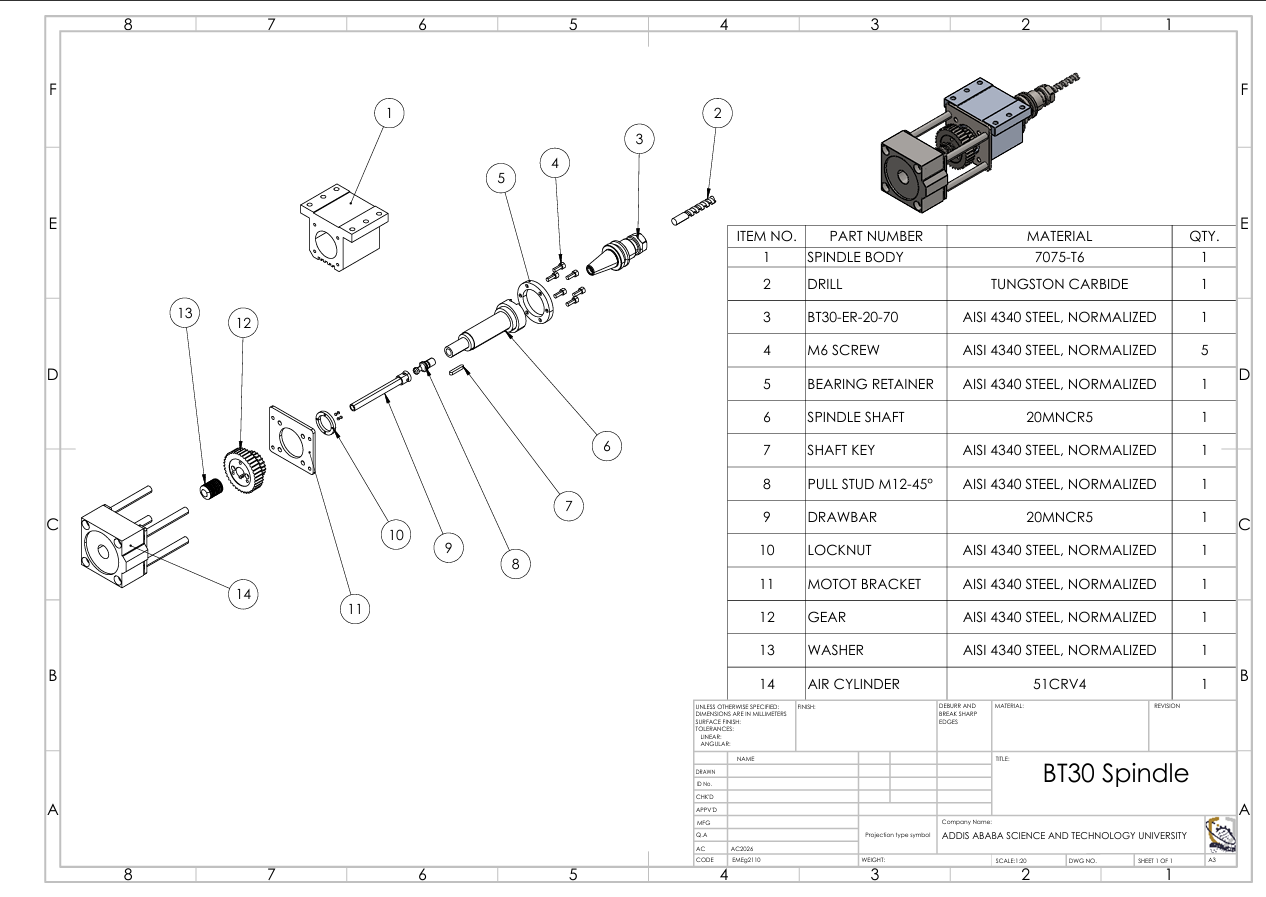
\includegraphics[width=\textwidth]{Pictures/2d_drawing.png}
			\caption{SolidWorks 2D engineering drawing.}
			\label{fig:2d_drawing}
		\end{figure}
		
		\chapter{MATLAB Scripts}
		
		\section{CNC Spindle Speed-Loop Control Design}
		
		\begin{lstlisting}
			%% ========================================================================
			%  CNC Spindle Speed-Loop Control Design
			%  Section 3.5/3.6 companion script: plant modeling, PID design via pole
			%  placement, root locus, Bode stability margins, closed-loop step response.
			% =========================================================================
			
			clear; clc; close all;
			
			%% ---------------------------------------------------------------------
			%  1. PLANT PARAMETERS
			%  Mechanical parameters are motor-shaft-referred: the spindle-side shaft,
			%  pulley, and tool-holder inertia are reflected through the measured
			%  ~1.70:1 belt ratio (spindle:motor) before being lumped into J.
			%  Electrical parameters are TYPICAL values for a 1 kW / 110 V AC servo
			%  class motor -- ASSUMED pending a specific manufacturer datasheet.
			% ------------------------------------------------------------------------
			J  = 5.45e-4;   % kg.m^2   total inertia, motor-shaft-referred
			B  = 5.00e-4;   % N.m.s/rad  viscous friction (assumed)
			R  = 2.0;       % ohm        phase resistance (assumed, typical 1kW AC servo)
			L  = 0.008;     % H          phase inductance (assumed, typical 1kW AC servo)
			Kt = 0.35;      % N.m/A      torque constant  (assumed, typical 1kW AC servo)
			Ke = 0.35;      % V.s/rad    back-EMF constant (= Kt in SI units)
			
			fprintf('=== PLANT PARAMETERS ===\n');
			fprintf('J=%.4e kg.m^2, B=%.4e N.m.s/rad\n', J, B);
			fprintf('R=%.2f ohm, L=%.4f H, Kt=Ke=%.2f\n\n', R, L, Kt);
			
			%% ---------------------------------------------------------------------
			%  2. PLANT TRANSFER FUNCTION  G(s) = Omega(s)/V(s)
			%     Combines mechanical: J*w_dot = Tm - TL - B*w,  Tm = Kt*I
			%     with electrical:     V = I*R + L*I_dot + Ke*w
			%     Eliminating I(s):    G(s) = Kt / [ (Js+B)(Ls+R) + Kt*Ke ]
			% ------------------------------------------------------------------------
			a2 = J*L;
			a1 = J*R + B*L;
			a0 = B*R + Kt*Ke;
			
			G = tf(Kt, [a2 a1 a0]);
			fprintf('=== PLANT TRANSFER FUNCTION G(s) ===\n');
			
			p_ol = pole(G);
			[wn_ol, zeta_ol] = damp(G);
			fprintf('Open-loop poles: %.3f %+.3fj , %.3f %+.3fj\n', ...
			real(p_ol(1)), imag(p_ol(1)), real(p_ol(2)), imag(p_ol(2)));
			fprintf('Natural frequency wn = %.2f rad/s, damping ratio zeta = %.4f\n', ...
			wn_ol(1), zeta_ol(1));
			fprintf('DC gain G(0) = %.4f (rad/s)/V\n\n', dcgain(G));
			
			%% ---------------------------------------------------------------------
			%  3. DESIRED CLOSED-LOOP DYNAMICS -> DOMINANT POLE LOCATIONS
			%     ts  = 2%% settling time target
			%     OS  = overshoot target (fractional, e.g. 0.05 = 5%%)
			% ------------------------------------------------------------------------
			ts = 0.05;      % seconds
			OS = 0.05;      % 5% overshoot
			
			zeta = -log(OS) / sqrt(pi^2 + log(OS)^2);
			wn   = 4 / (zeta*ts);
			
			p1 = complex(-zeta*wn,  wn*sqrt(1-zeta^2));
			p2 = conj(p1);
			p3 = -5*abs(real(p1));   % non-dominant 3rd pole, placed far left
			
			fprintf('=== DESIRED CLOSED-LOOP POLES ===\n');
			fprintf('Target zeta = %.4f, wn = %.2f rad/s\n', zeta, wn);
			fprintf('Dominant poles: %.2f %+.2fj\n', real(p1), imag(p1));
			fprintf('Non-dominant pole: %.2f\n\n', p3);
			
			desired_poly = poly([p1 p2 p3]);   % monic cubic: s^3 + c2 s^2 + c1 s + c0
			desired_poly = real(desired_poly);
			c2 = desired_poly(2); c1 = desired_poly(3); c0 = desired_poly(4);
			
			%% ---------------------------------------------------------------------
			%  4. PID GAINS VIA POLE PLACEMENT
			%     Closed-loop char. eq. (unity feedback, C(s) = (Kd s^2+Kp s+Ki)/s):
			%     a2 s^3 + (a1+Kt*Kd) s^2 + (a0+Kt*Kp) s + Kt*Ki = 0
			%     Normalize by a2 and match coefficients to the desired monic cubic.
			% ------------------------------------------------------------------------
			Kd = (c2*a2 - a1) / Kt;
			Kp = (c1*a2 - a0) / Kt;
			Ki = (c0*a2) / Kt;
			
			fprintf('=== PID GAINS (pole placement) ===\n');
			fprintf('Kp = %.4f\nKi = %.2f\nKd = %.6f\n\n', Kp, Ki, Kd);
			
			C  = tf([Kd Kp Ki], [1 0]);      % PID controller C(s)
			L_ol = series(C, G);              % open-loop C(s)G(s)
			T_cl = feedback(L_ol, 1);         % closed-loop, unity feedback
			
			p_cl = pole(T_cl);
			fprintf('Closed-loop poles (verification, should match Section 3 target):\n');
			disp(p_cl);
			
			%% ---------------------------------------------------------------------
			%  5. LEAD/LAG CHARACTER OF THE DESIGNED PID
			%     C(s) = Kd*(s^2 + (Kp/Kd)s + (Ki/Kd)) / s
			%     The /s term is a pure LAG (integrator) providing zero steady-state
			%     error; the numerator's complex zero pair provides LEAD (phase
			%     recovery) near crossover to compensate for the ~90 deg of phase the
			%     integrator removes. A PID is therefore a combined lag-lead design.
			% ------------------------------------------------------------------------
			b1 = Kp/Kd; b0 = Ki/Kd;
			disc = b1^2 - 4*b0;
			fprintf('\n=== PID ZERO ANALYSIS (lead/lag character) ===\n');
			if disc < 0
			zr = -b1/2; zi = sqrt(-disc)/2;
			wn_z = sqrt(b0); zeta_z = b1/(2*wn_z);
			fprintf('Complex zero pair: %.2f +/- %.2fj\n', zr, zi);
			fprintf('Zero-pair wn=%.2f rad/s, zeta=%.3f (LEAD action near crossover)\n', wn_z, zeta_z);
			else
			zr = roots([1 b1 b0]);
			fprintf('Real zeros: %.2f, %.2f\n', zr(1), zr(2));
			end
			fprintf('Pole at origin (1/s): pure LAG / integral action (zero steady-state error)\n\n');
			
			%% ---------------------------------------------------------------------
			%  6. STABILITY MARGINS
			% ------------------------------------------------------------------------
			[Gm, Pm, Wcg, Wcp] = margin(L_ol);
			fprintf('=== STABILITY MARGINS (open loop C(s)G(s)) ===\n');
			if isinf(Gm)
			fprintf('Gain margin: Inf dB\n');
			else
			fprintf('Gain margin: %.2f dB at %.1f rad/s\n', 20*log10(Gm), Wcg);
			end
			fprintf('Phase margin: %.1f deg at %.1f rad/s (crossover)\n\n', Pm, Wcp);
			
			%% ---------------------------------------------------------------------
			%  7. ROOT LOCUS  (fixed PID zero/pole SHAPE, varying overall gain K)
			%     K = Kd is our actual design point; the locus shows how the closed-
			%     loop poles migrate for other gains along the same compensator shape.
			% ------------------------------------------------------------------------
			shape = tf([1 b1 b0], [1 0]);     % PID shape normalized to unit leading coeff
			OL_shape = series(shape, G);       % K * shape * G is the swept open loop
			
			k_vec = [0 logspace(-4, 1, 4000)];   % 0 up to K=10, well beyond K=Kd, in fine steps
			fig1 = figure('Name','Root Locus');
			[r, k] = rlocus(OL_shape, k_vec);
			plot(real(r).', imag(r).', 'b-');
			hold on;
			plot(real(p_cl), imag(p_cl), 'r*', 'MarkerSize', 14, 'LineWidth', 2);
			p_ol_shape = pole(OL_shape);
			z_ol_shape = zero(OL_shape);
			plot(real(p_ol_shape), imag(p_ol_shape), 'bx', 'MarkerSize', 10);
			plot(real(z_ol_shape), imag(z_ol_shape), 'bo', 'MarkerSize', 10);
			hold off;
			grid on;
			xlim([-450 50]);      % zoom to the physically meaningful region
			ylim([-150 150]);
			xlabel('Real Axis (1/s)'); ylabel('Imaginary Axis (1/s)');
			title('Root Locus: PID-shaped open loop C(s)G(s)/K_d vs gain K');
			legend({'Root locus branches','Design point (K=K_d)','Open-loop poles','Open-loop zeros'}, ...
			'Location','best');
			saveas(fig1, 'Pictures/root_locus_matlab.png');
			
			%% ---------------------------------------------------------------------
			%  8. BODE PLOT WITH MARGINS
			% ------------------------------------------------------------------------
			fig2 = figure('Name','Bode with Margins');
			margin(L_ol);
			grid on;
			saveas(fig2, 'Pictures/bode_margins_matlab.png');
			
			%% ---------------------------------------------------------------------
			%  9. CLOSED-LOOP STEP RESPONSE
			% ------------------------------------------------------------------------
			fig3 = figure('Name','Closed-Loop Step Response');
			step(T_cl, 0.1);
			grid on;
			title('Closed-loop speed step response (verification of PID design)');
			saveas(fig3, 'Pictures/step_response_matlab.png');
			
			info = stepinfo(T_cl);
			fprintf('=== STEP RESPONSE CHARACTERISTICS ===\n');
			fprintf('Rise time:     %.4f s\n', info.RiseTime);
			fprintf('Settling time: %.4f s\n', info.SettlingTime);
			fprintf('Overshoot:     %.2f %%\n', info.Overshoot);
			fprintf('Peak:          %.4f\n', info.Peak);
			
			%% ---------------------------------------------------------------------
			% 10. DISTURBANCE REJECTION CHECK
			%
			%     Step response of the closed-loop speed to a cutting-torque step of
			%     magnitude TL_nominal. The time axis starts at the moment the step
			%     is applied, so this is a design-verification curve -- it shows the
			%     shape and magnitude of the speed dip and recovery, not the timing
			%     of the t = 0.1 s load transient in the full plant simulation.
			%
			%     Transfer function from TL to Omega at the plant input side:
			%       Omega(s)/TL(s) = -(Ls+R) / [(Js+B)(Ls+R)+Kt*Ke]   (open loop)
			%     The disturbance enters at the same summing point as V, so the
			%     closed-loop path is shaped by the sensitivity function S(s), not
			%     by feedback(Gtl, C).
			% ------------------------------------------------------------------------
			Gtl = tf(-[L R], [a2 a1 a0]);          % TL -> Omega, open-loop plant path
			S   = feedback(1, L_ol);                % sensitivity function 1/(1+L_ol)
			Gtl_cl = Gtl * S;                       % disturbance shaped by S(s)
			
			% Peak cutting torque (Section 3.1.1.3). Same value used in Scripts 1
			% and 2; named TL_nominal to keep vocabulary consistent across the three
			% companion scripts.
			TL_nominal = 0.675;    % N.m
			
			t = 0:0.0005:0.15;
			fig4 = figure('Name','Disturbance Rejection (torque step)');
			step(TL_nominal*Gtl_cl, t);
			grid on;
			title('Speed dip and recovery under a step cutting-torque disturbance');
			xlabel('Time (s) after disturbance onset'); ylabel('\Delta\Omega (rad/s)');
			saveas(fig4, 'Pictures/disturbance_rejection_matlab.png');
			
			fprintf('\nDone. Figures saved: Pictures/root_locus_matlab.png, Pictures/bode_margins_matlab.png,\n');
			fprintf('Pictures/step_response_matlab.png, Pictures/disturbance_rejection_matlab.png\n');
		\end{lstlisting}
		
		\section{CNC Milling Spindle -- PLC Supervisory Interlock Simulation}
		
		\begin{lstlisting}
			%% ========================================================================
			% CNC Milling Spindle - PLC Supervisory Interlock Simulation
			%
			% Project:
			% Design, Analysis, and Modeling of a CNC Milling Spindle System
			%
			% Purpose:
			% Compare tool-change operation:
			%   1. Without PLC supervisory interlock
			%   2. With PLC supervisory interlock
			%
			% The existing PID speed controller remains responsible for spindle-speed
			% regulation. The PLC/Stateflow logic is represented here as supervisory
			% discrete logic that controls the safe sequence for tool release.
			%
			% ========================================================================
			
			clear;
			clc;
			close all;
			
			%% ========================================================================
			% 1. SPINDLE AND MOTOR PARAMETERS
			% ========================================================================
			
			J  = 5.45e-4;      % kg.m^2, total rotational inertia
			B  = 5.00e-4;      % N.m.s/rad, viscous friction
			R  = 2.0;          % ohm, phase resistance
			L  = 0.008;        % H, phase inductance
			
			Kt = 0.35;         % N.m/A, torque constant
			Ke = 0.35;         % V.s/rad, back-EMF constant
			
			%% ========================================================================
			% 2. PID CONTROLLER
			%    Values obtained from the existing pole-placement design.
			%
			%    NOTE: the pid() object is not built here because the main loop
			%    implements the controller directly (needed for the reference filter,
			%    D-on-measurement, and conditional-integration anti-windup). If you
			%    want the Control System Toolbox object for a design check, uncomment
			%    the line below.
			% ========================================================================
			
			Kp = 0.6118;
			Ki = 66.96;
			Kd = 0.003850;
			
			% C_PID = pid(Kp, Ki, Kd);   % kept out of the loop, see note above
			
			%% ========================================================================
			% 3. SPINDLE PLANT
			%
			% Electrical:
			%       V = R I + L dI/dt + Ke*w
			%
			% Mechanical:
			%       J dw/dt = Kt I - B*w - TL
			%
			% State vector:
			%       x = [I  w]'
			%
			% Inputs:
			%       u = [V  TL]'
			%
			% Output:
			%       y = w
			% ========================================================================
			
			A = [-R/L      -Ke/L;
			Kt/J     -B/J];
			
			Bplant = [1/L       0;
			0        -1/J];
			
			Cplant = [0 1];
			
			Dplant = [0 0];
			
			Plant = ss(A, Bplant, Cplant, Dplant);   % kept for reference / design check
			
			%% ========================================================================
			% 3b. NOMINAL CUTTING TORQUE
			% ========================================================================
			
			% Peak cutting torque used throughout the simulation. Matches the value
			% used in the Simulink model and the pole-placement design report.
			
			TL_nominal = 0.675;    % N.m
			
			%% ========================================================================
			% 4. OPERATING CONDITIONS
			% ========================================================================
			
			RPM_nominal = 5000;
			
			% Convert RPM to rad/s
			omega_nominal = RPM_nominal * 2*pi/60;
			
			% Tool-change request time
			t_request = 0.10;       % s
			
			% Simulation duration
			t_end = 0.30;           % s
			
			% Time step
			dt = 1e-4;              % s
			
			t = (0:dt:t_end)';
			
			%% ========================================================================
			% 5. TOOL-CHANGE STOPPING CONDITION
			% ========================================================================
			
			% The spindle is considered stationary when its speed falls below this
			% threshold.
			
			RPM_stop_threshold = 5;          % rpm
			omega_stop_threshold = ...
			RPM_stop_threshold * 2*pi/60;
			
			%% ========================================================================
			% 6. TOOL-CHANGE REQUEST
			% ========================================================================
			
			Tool_Change_Request = double(t >= t_request);
			
			%% ========================================================================
			% 7. INITIAL CONDITIONS
			% ========================================================================
			
			% Assume spindle is initially operating at 5000 RPM.
			
			x = zeros(2,1);
			
			% Loaded steady-state current: viscous friction torque + cutting torque
			I_initial = (B*omega_nominal + TL_nominal) / Kt;
			
			x(1) = I_initial;
			x(2) = omega_nominal;
			
			%% ========================================================================
			% 7b. STEADY-STATE FEEDFORWARD VOLTAGE
			%
			% Voltage required to hold the nominal speed against the nominal cutting
			% load. Supplying this directly at the plant input keeps the PID's
			% integrator from having to carry the DC operating point, which eliminates
			% the startup dip and matches the Simulink model.
			% ========================================================================
			
			V_ss = R*I_initial + Ke*omega_nominal;    % ~188.6 V
			
			%% ========================================================================
			% 8. PID STATE VARIABLES
			% ========================================================================
			
			integral_error  = 0;
			omega_previous  = omega_nominal;     % for D-on-measurement
			
			%% ========================================================================
			% 8b. REFERENCE LOW-PASS FILTER
			%
			% A first-order filter is applied to the PLC speed command before it
			% reaches the PID. Without this filter, the step from 5000 RPM to 0 rpm
			% at t_request produces a large derivative kick (Kd * d(error)/dt) on the
			% voltage command.
			%
			% The filter time constant is chosen much smaller than the closed-loop
			% settling time so that it does not slow the response, but large enough
			% to round off the hard step.
			% ========================================================================
			
			tau_ref        = 0.005;              % s, reference filter time constant
			omega_ref_filt = omega_nominal;      % scalar running filter state
			
			%% ========================================================================
			% 9. SIMULATION ARRAYS
			% ========================================================================
			
			omega = zeros(size(t));
			RPM   = zeros(size(t));
			
			omega_ref_cmd  = zeros(size(t));     % pre-filter reference (rad/s)
			omega_ref_used = zeros(size(t));     % post-filter reference (rad/s)
			
			Voltage_command = zeros(size(t));
			
			Cylinder_nonPLC = zeros(size(t));
			Cylinder_PLC    = zeros(size(t));
			
			PLC_Stop_Command = zeros(size(t));
			PLC_State_signal = zeros(size(t));   % logged every step (see Section 12)
			
			%% ========================================================================
			% 10. NON-PLC CASE
			%
			% In this case the tool-release command is generated directly from the
			% tool-change request.
			%
			% Therefore:
			%
			% Tool Change Request = 1
			%             |
			%             v
			%     Cylinder Actuate
			%
			% The cylinder can fire while the spindle is still rotating.
			% ========================================================================
			
			Cylinder_nonPLC(t >= t_request) = 1;
			
			%% ========================================================================
			% 11. PLC SUPERVISORY LOGIC
			%
			% State sequence:
			%
			% NORMAL OPERATION
			%       |
			%       | Tool Change Request
			%       v
			% STOPPING
			%       |
			%       | RPM <= stopping threshold
			%       v
			% TOOL RELEASE
			%       |
			%       | Drawbar delay AND RPM still <= stopping threshold
			%       v
			% NORMAL / TOOL CHANGE COMPLETE
			%
			% The PLC does NOT replace the PID controller.
			% It changes the permitted spindle reference and controls the tool-release
			% permission.
			%
			% NOTE (bug fix carried over from the previous revision):
			% The original logic latched the "stopping threshold reached" condition at
			% the moment of entering the RELEASE state and then fired the cylinder
			% after a fixed delay without re-checking the speed. Because the PID
			% integral action could push the speed back above the threshold during
			% that delay, the tool could still be released at an unsafe speed.
			%
			% The corrected logic re-checks the speed inside the RELEASE state. If
			% the speed has risen above the threshold, the PLC returns to STOPPING
			% and the delay timer is reset.
			% ========================================================================
			
			PLC_STATE_NORMAL   = 0;
			PLC_STATE_STOPPING = 1;
			PLC_STATE_RELEASE  = 2;
			PLC_STATE_COMPLETE = 3;
			
			PLC_State = PLC_STATE_NORMAL;
			
			release_delay = 0.020;       % s, simulated drawbar actuation delay
			release_timer = 0;
			
			%% ========================================================================
			% 12. MAIN CLOSED-LOOP SIMULATION
			% ========================================================================
			
			V_max = 325;    % V, full-wave-rectified peak of the 230 V single-phase mains (230*sqrt(2))
			
			for k = 1:length(t)
			
			%% ---------------------------------------------------------------
			% Current spindle speed
			% ---------------------------------------------------------------
			
			omega(k) = x(2);
			RPM(k)   = omega(k) * 60/(2*pi);
			
			%% ---------------------------------------------------------------
			% PLC SUPERVISORY LOGIC
			% ---------------------------------------------------------------
			
			if Tool_Change_Request(k) == 0
			
			% Normal machining
			PLC_State = PLC_STATE_NORMAL;
			
			else
			
			switch PLC_State
			
			case PLC_STATE_NORMAL
			
			% Tool change requested
			PLC_State = PLC_STATE_STOPPING;
			
			case PLC_STATE_STOPPING
			
			% Command spindle to stop
			PLC_Stop_Command(k) = 1;
			
			% Wait until spindle reaches stopping threshold
			if abs(RPM(k)) <= RPM_stop_threshold
			
			PLC_State = PLC_STATE_RELEASE;
			release_timer = t(k);
			end
			
			case PLC_STATE_RELEASE
			
			PLC_Stop_Command(k) = 1;
			
			% ---- BUG FIX -----------------------------------------
			% Re-check the speed at every step while waiting for the
			% drawbar delay. If the spindle has sped back up, we are
			% no longer safe to release the tool.
			% -----------------------------------------------------
			if abs(RPM(k)) > RPM_stop_threshold
			
			% Speed is no longer safe: go back to stopping and
			% restart the release timer.
			PLC_State = PLC_STATE_STOPPING;
			release_timer = 0;
			
			elseif (t(k) - release_timer) >= release_delay
			
			% Drawbar delay elapsed AND speed is still safe.
			Cylinder_PLC(k) = 1;
			PLC_State = PLC_STATE_COMPLETE;
			
			end
			
			case PLC_STATE_COMPLETE
			
			PLC_Stop_Command(k) = 1;
			Cylinder_PLC(k)     = 1;
			
			end
			end
			
			% Log the state every step for Figure 4 (no post-hoc reconstruction).
			PLC_State_signal(k) = PLC_State;
			
			%% ---------------------------------------------------------------
			% PLC-GENERATED SPEED REFERENCE (rad/s)
			% ---------------------------------------------------------------
			
			if PLC_State == PLC_STATE_NORMAL
			omega_ref_cmd(k) = omega_nominal;   % run at nominal speed
			else
			omega_ref_cmd(k) = 0;               % tool change -> stop
			end
			
			%% ---------------------------------------------------------------
			% REFERENCE LOW-PASS FILTER
			%
			% First-order update:
			%       w_f[k+1] = w_f[k] + (dt/tau_ref) * (w_cmd[k] - w_f[k])
			% ---------------------------------------------------------------
			
			omega_ref_filt = omega_ref_filt + (dt/tau_ref) * ...
			(omega_ref_cmd(k) - omega_ref_filt);
			
			omega_ref_used(k) = omega_ref_filt;
			
			%% ---------------------------------------------------------------
			% PID SPEED CONTROLLER
			%
			%   P  : on speed error
			%   I  : on speed error (with conditional-integration anti-windup)
			%   D  : on measurement only (avoids derivative kick on the step)
			% ---------------------------------------------------------------
			
			error = omega_ref_used(k) - omega(k);
			
			% Integral term
			integral_error = integral_error + error*dt;
			
			% Derivative term on measurement (note the negative sign, because
			% d(error)/dt = -d(omega)/dt when the reference is (locally) constant).
			derivative_meas = -(omega(k) - omega_previous)/dt;
			omega_previous  = omega(k);
			
			% PID output (unsaturated)
			V_unsat = Kp*error + Ki*integral_error + Kd*derivative_meas;
			
			% Feedforward + feedback -> total actuator demand
			V_total_unsat = V_unsat + V_ss;
			
			% Saturation on the total command (physically correct single-saturation
			% architecture: the DC bus limit applies to the sum).
			V = max(min(V_total_unsat, V_max), -V_max);
			
			% Conditional-integration anti-windup on the total command
			if (V_total_unsat >  V_max && error > 0) || ...
			(V_total_unsat < -V_max && error < 0)
			integral_error = integral_error - error*dt;
			end
			
			Voltage_command(k) = V;
			
			%% ---------------------------------------------------------------
			% CUTTING TORQUE
			%
			% Cutting torque is removed when tool-change operation begins.
			% ---------------------------------------------------------------
			
			if Tool_Change_Request(k) == 0
			TL = TL_nominal;
			else
			TL = 0;
			end
			
			%% ---------------------------------------------------------------
			% PLANT DYNAMICS
			% ---------------------------------------------------------------
			
			dx = A*x + Bplant*[V; TL];
			x  = x + dx*dt;
			
			% ---- One-way bearing physical constraint ------------------------
			% The spindle cannot rotate in reverse. If numerical integration
			% produces a negative speed, clamp at zero.
			% ----------------------------------------------------------------
			if x(2) < 0
			x(2) = 0;
			end
			
			end
			
			%% ========================================================================
			% 13. ENSURE FINAL VALUES ARE RECORDED
			% ========================================================================
			
			omega(end) = x(2);
			RPM(end)   = omega(end)*60/(2*pi);
			
			%% ========================================================================
			% 14. SAFETY CHECK
			% ========================================================================
			
			% Find the first instant at which the PLC permits cylinder actuation.
			
			idx_release = find(Cylinder_PLC > 0,1,'first');
			
			if ~isempty(idx_release)
			
			release_time = t(idx_release);
			release_RPM  = RPM(idx_release);
			
			else
			
			release_time = NaN;
			release_RPM  = NaN;
			
			end
			
			%% ========================================================================
			% 15. UNSAFE RELEASE CHECK
			% ========================================================================
			
			idx_nonPLC = find(Cylinder_nonPLC > 0,1,'first');
			
			unsafe_release_time = t(idx_nonPLC);
			unsafe_release_RPM  = RPM(idx_nonPLC);
			
			%% ========================================================================
			% 16. DISPLAY RESULTS
			% ========================================================================
			
			fprintf('\n');
			fprintf('============================================================\n');
			fprintf(' CNC SPINDLE TOOL-CHANGE INTERLOCK SIMULATION\n');
			fprintf('============================================================\n');
			
			fprintf('\nInitial spindle speed: %.1f RPM\n', RPM_nominal);
			
			fprintf('\nWITHOUT PLC INTERLOCK:\n');
			fprintf('Cylinder release time: %.4f s\n', unsafe_release_time);
			fprintf('Spindle speed at release: %.2f RPM\n', unsafe_release_RPM);
			
			fprintf('\nWITH PLC INTERLOCK:\n');
			fprintf('Cylinder release time: %.4f s\n', release_time);
			fprintf('Spindle speed at release: %.2f RPM\n', release_RPM);
			
			fprintf('\nStopping threshold: %.2f RPM\n', RPM_stop_threshold);
			
			% Extra explicit safety assertion for the report
			if ~isnan(release_RPM)
			if abs(release_RPM) <= RPM_stop_threshold
			fprintf('Safety check: PASS - PLC release speed is within threshold.\n');
			else
			fprintf('Safety check: FAIL - PLC release speed is above threshold.\n');
			end
			end
			
			%% ========================================================================
			% 17. FIGURE 1 - SPINDLE SPEED AND TOOL-CHANGE REQUEST
			% ========================================================================
			
			figure('Name','Spindle Speed During Tool Change');
			
			yyaxis left
			
			plot(t,RPM,'LineWidth',1.5);
			hold on;
			
			% Filtered reference (post-LPF) is what the PID actually tracks.
			plot(t,omega_ref_used * 60/(2*pi),'--','LineWidth',1.2);
			
			yline(RPM_stop_threshold,':','Stopping Threshold');
			
			ylabel('Spindle Speed (RPM)');
			
			yyaxis right
			
			plot(t,Tool_Change_Request,'LineWidth',1.2);
			
			ylabel('Tool Change Request');
			
			xlabel('Time (s)');
			title('CNC Spindle Speed During Tool-Change Sequence');
			
			grid on;
			
			legend('Actual RPM',...
			'PLC Commanded RPM (filtered)',...
			'Stopping Threshold',...
			'Tool Change Request',...
			'Location','best');
			
			%% ========================================================================
			% 18. FIGURE 2 - NON-PLC VS PLC CYLINDER ACTUATION
			% ========================================================================
			
			figure('Name','PLC Interlock Comparison');
			
			plot(t,RPM/1000,'LineWidth',1.5);
			hold on;
			
			plot(t,Cylinder_nonPLC*5,'--','LineWidth',1.5);
			
			plot(t,Cylinder_PLC*5,'-.','LineWidth',1.5);
			
			yline(RPM_stop_threshold/1000,':');
			
			xlabel('Time (s)');
			ylabel('Speed / Actuator State');
			
			title('Comparison of Tool-Release Operation');
			
			legend('Spindle Speed (1000 RPM)',...
			'Cylinder - No PLC',...
			'Cylinder - PLC Interlock',...
			'Stopping Threshold',...
			'Location','best');
			
			grid on;
			
			%% ========================================================================
			% 19. FIGURE 3 - SAFETY TIMELINE (5 PANELS)
			%
			% Extra panel added: the PLC Stop Command is now shown explicitly so the
			% reader can see the supervisory command separate from the cylinder firing.
			% ========================================================================
			
			figure('Name','Tool Change Safety Timeline');
			
			subplot(5,1,1);
			plot(t,RPM,'LineWidth',1.5);
			hold on;
			yline(RPM_stop_threshold,':');
			ylabel('RPM');
			title('Tool-Change Safety Sequence');
			grid on;
			
			subplot(5,1,2);
			stairs(t,Tool_Change_Request,'LineWidth',1.5);
			ylim([-0.1 1.1]);
			ylabel('Request');
			grid on;
			
			subplot(5,1,3);
			stairs(t,PLC_Stop_Command,'LineWidth',1.5);
			ylim([-0.1 1.1]);
			ylabel('PLC Stop');
			grid on;
			
			subplot(5,1,4);
			stairs(t,Cylinder_nonPLC,'LineWidth',1.5);
			ylim([-0.1 1.1]);
			ylabel('No PLC');
			grid on;
			
			subplot(5,1,5);
			stairs(t,Cylinder_PLC,'LineWidth',1.5);
			ylim([-0.1 1.1]);
			ylabel('PLC');
			xlabel('Time (s)');
			grid on;
			
			%% ========================================================================
			% 20. FIGURE 4 - PLC STATE SEQUENCE
			%
			% The state sequence is now taken directly from PLC_State_signal, which
			% is logged during the simulation. This guarantees the plot reflects the
			% actual state machine execution (no post-hoc reconstruction that could
			% disagree with the logic).
			% ========================================================================
			
			figure('Name','PLC Supervisory State Sequence');
			
			stairs(t,PLC_State_signal,'LineWidth',1.8);
			
			yticks([0 1 2 3]);
			
			yticklabels({'NORMAL',...
				'STOPPING',...
				'RELEASE',...
				'COMPLETE'});
			
			xlabel('Time (s)');
			ylabel('PLC State');
			
			title('Supervisory PLC State Sequence');
			
			grid on;
			
			%% ========================================================================
			% 21. SAVE FIGURES FOR REPORT
			% ========================================================================
			
			saveas(figure(1),'Pictures/spindle_tool_change_speed.png');
			saveas(figure(2),'Pictures/plc_interlock_comparison.png');
			saveas(figure(3),'Pictures/tool_change_safety_timeline.png');
			saveas(figure(4),'Pictures/plc_state_sequence.png');
			
			%% ========================================================================
			% END OF SCRIPT
			% ========================================================================
		\end{lstlisting}
		
		\chapter{MATLAB/Simulink Block Diagrams}
		
		\begin{figure}[htbp]
			\centering
			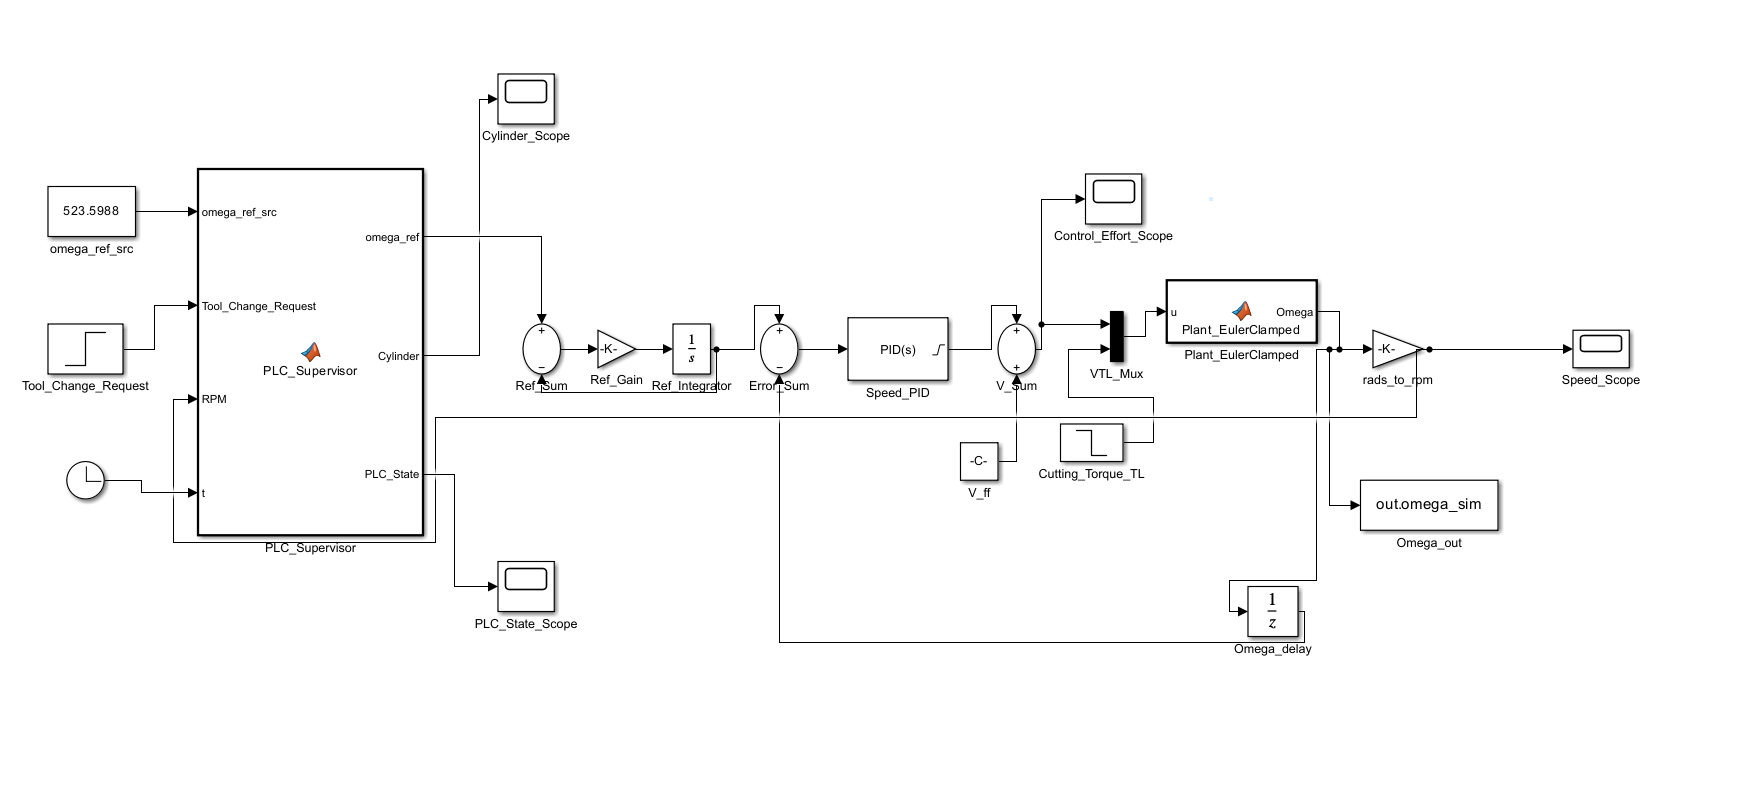
\includegraphics[width=\textwidth]{Pictures/simulink_diagram.png}
			\caption{MATLAB/Simulink block diagram.}
			\label{fig:simulink_diagram}
		\end{figure}
		
	\end{document}